% Fichier généré à partir de rapport_volet1_final.md et des images extraites de rapport_volet1_final.docx.
\section{Volet 1 : Conteneurisation Docker et Docker Swarm}

\textbf{Conteneurisation et Orchestration des Conteneurs}



\subsection{Introduction}

Ce rapport présente le travail réalisé dans le cadre du Volet 1 du mini-projet NeoTech, qui consiste en la conteneurisation de l'application web 3-tiers \textbf{Travelo} (React, Spring Boot, MySQL) à l'aide de Docker, ainsi que son déploiement en mode cluster avec Docker Swarm.



\subsection{1. Création du réseau Docker}

Un réseau Docker dédié est créé avec le driver bridge afin d'isoler les conteneurs et permettre leur communication par nom de service.

\begin{lstlisting}[language=bash]
docker network create --driver bridge travelo-network
\end{lstlisting}

\begin{figure}[H]
    \centering
    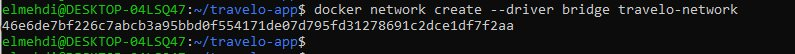
\includegraphics[width=0.95\textwidth]{./screenshots/volet1/01_creation_reseau_docker_travelo-network.png}
    \caption{Création du réseau Docker "travelo-network" avec le driver bridge}
\end{figure}

Le driver bridge est le choix le plus adapté pour une utilisation locale (single host) : il crée un réseau virtuel isolé sur la machine hôte, permettant la communication entre conteneurs via leur nom.



\subsection{2. Création du conteneur MySQL avec stockage persistant}

\subsubsection{2.a. Volume Docker pour la persistance}

Le stockage des données MySQL est rendu persistant via un volume Docker nommé, garantissant l'indépendance des données par rapport au cycle de vie du conteneur.

\begin{lstlisting}[language=bash]
docker volume create travelo_mysql_data
\end{lstlisting}

\begin{figure}[H]
    \centering
    
\includegraphics[width=0.95\textwidth]{./screenshots/volet1/02_creation_volume_docker_travelo_mysql_data.png}
    \caption{Création du volume Docker "travelo\_mysql\_data"}
\end{figure}

\subsubsection{2.b. Lancement du conteneur MySQL}

\begin{lstlisting}[language=bash]
docker run -d --name travelo_app --network travelo-network \
  -v travelo_mysql_data:/var/lib/mysql \
  -e MYSQL_ROOT_PASSWORD=password -e MYSQL_DATABASE=travelo_db \
  mysql:8
\end{lstlisting}

\begin{itemize}
    \item \texttt{-d} : Mode détaché
    \item \texttt{--name} : Nom du conteneur
    \item \texttt{--network} : Réseau partagé
    \item \texttt{-v} : Volume persistant
    \item \texttt{-e} : Variables d'environnement
\end{itemize}

\begin{figure}[H]
    \centering
    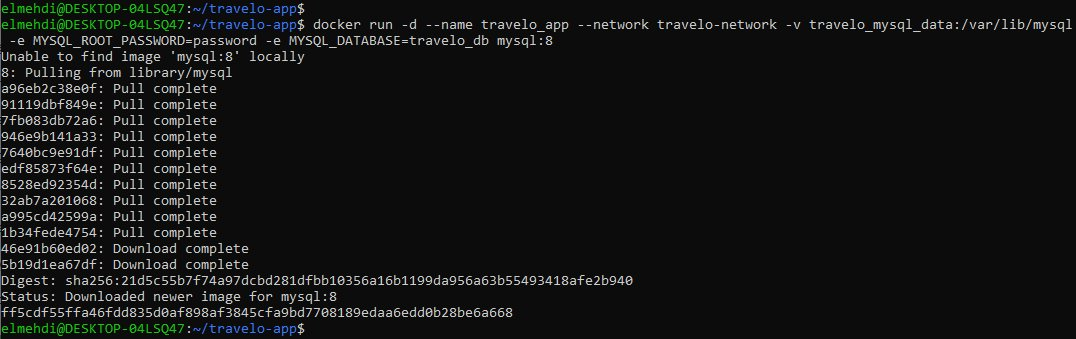
\includegraphics[width=0.95\textwidth]{./screenshots/volet1/03_lancement_conteneur_mysql_pull_demarrage.png}
    \caption{Lancement du conteneur MySQL (pull et démarrage de mysql:8)}
\end{figure}

\begin{figure}[H]
    \centering
    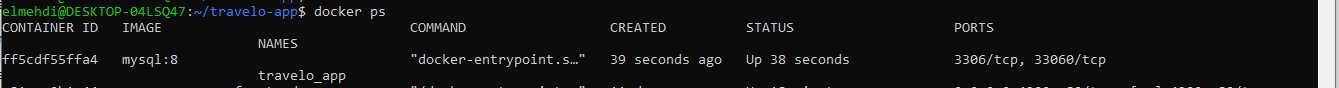
\includegraphics[width=0.95\textwidth]{./screenshots/volet1/04_docker_ps_conteneur_mysql_travelo_app_actif.png}
    \caption{\texttt{docker ps} : conteneur MySQL "travelo\_app" actif}
\end{figure}

\begin{figure}[H]
    \centering
    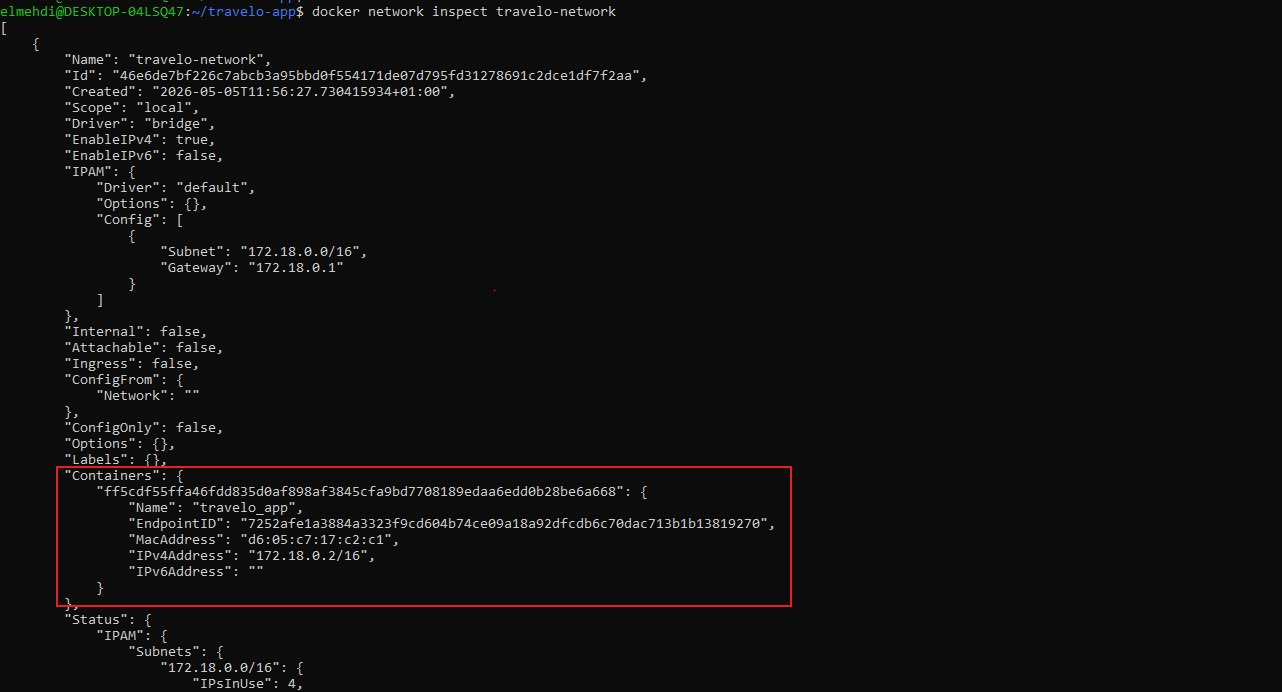
\includegraphics[width=0.95\textwidth]{./screenshots/volet1/05_inspection_reseau_travelo-network_mysql_connecte.png}
    \caption{Inspection du réseau travelo-network : conteneur MySQL connecté}
\end{figure}



\subsection{3. Dockerfile Backend – Bonnes pratiques}

\begin{figure}[H]
    \centering
    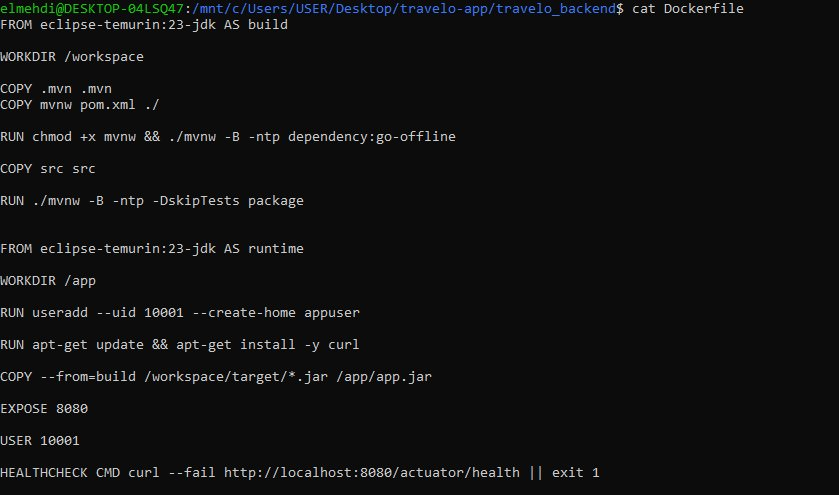
\includegraphics[width=0.95\textwidth]{./screenshots/volet1/06_dockerfile_backend_multistage_build_jdk23.png}
    \caption{Contenu du Dockerfile Backend (multi-stage build, JDK 23)}
\end{figure}



\subsection{4. Explication des bonnes pratiques}

\subsubsection{a. Multi-stage build}

Deux étapes distinctes : "build" (compilation Maven) et "runtime" (image légère). L'image finale exclut les outils de build, réduisant sa taille.

\subsubsection{b. Cache des dépendances Maven}

Copie séparée de \texttt{pom.xml} avant le code source pour exploiter le cache Docker : les dépendances ne sont retéléchargées que si \texttt{pom.xml} change.

\subsubsection{c. -DskipTests}

Les tests sont ignorés au build Docker ; ils sont exécutés séparément dans le pipeline CI/CD.

\subsubsection{d. Utilisateur non-root (UID 10001)}

Un utilisateur système \texttt{appuser} est créé pour exécuter l'application, respectant le principe du moindre privilège.

\subsubsection{e. HEALTHCHECK}

Surveillance de l'endpoint \texttt{/actuator/health} de Spring Boot pour que Docker monitore l'état de santé du conteneur.

\subsubsection{f. EXPOSE}

Documentation du port 8080 sans publication automatique sur l'hôte.



\subsection{5. Commandes Docker – Image Backend}

\subsubsection{5.a. Build de l'image}

\begin{lstlisting}[language=bash]
docker build -t travelo_backend_image .
\end{lstlisting}

\begin{figure}[H]
    \centering
    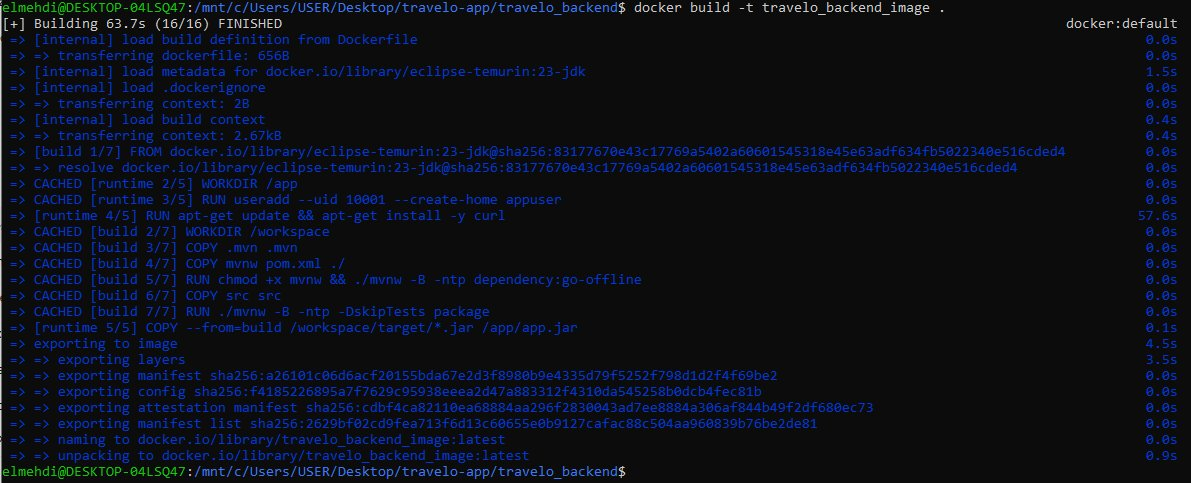
\includegraphics[width=0.95\textwidth]{./screenshots/volet1/07_build_backend_travelo_backend_image_succes.png}
    \caption{Build réussi de travelo\_backend\_image (16/16 étapes)}
\end{figure}

\begin{figure}[H]
    \centering
    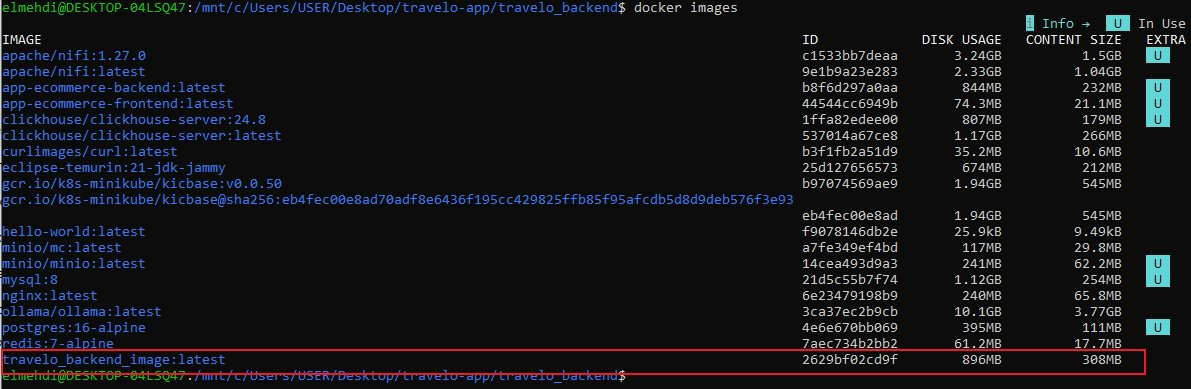
\includegraphics[width=0.95\textwidth]{./screenshots/volet1/08_docker_images_travelo_backend_image_896MB.png}
    \caption{\texttt{docker images} : travelo\_backend\_image:latest (896MB)}
\end{figure}

\subsubsection{5.b. Scan des vulnérabilités}

\begin{lstlisting}[language=bash]
trivy image --timeout 30m travelo_backend_image
\end{lstlisting}

405 vulnérabilités OS (Ubuntu 24.04) + 35 dans le JAR. Recommandation : utiliser \texttt{eclipse-temurin:23-jre-alpine} pour réduire la surface d'attaque.

\begin{figure}[H]
    \centering
    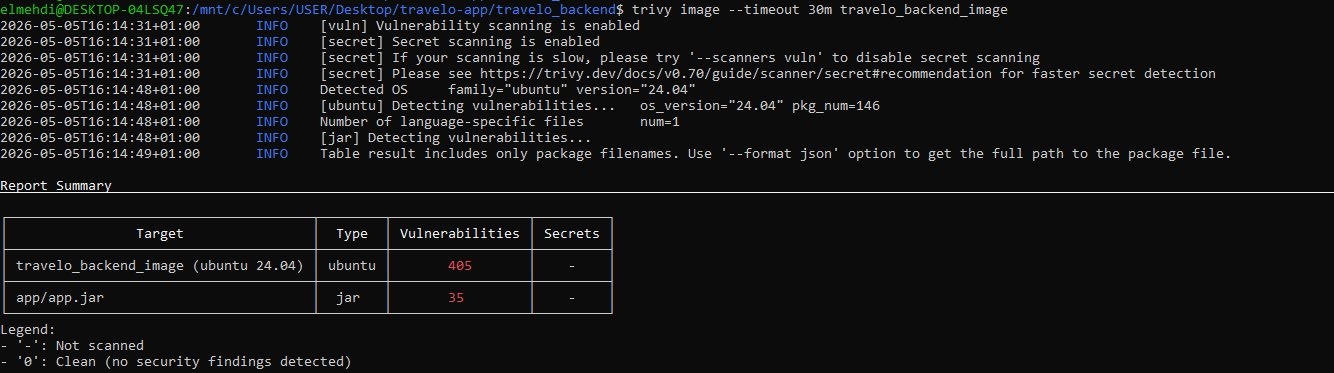
\includegraphics[width=0.95\textwidth]{./screenshots/volet1/09_trivy_scan_backend_405_vulnerabilites_OS_35_JAR.png}
    \caption{Trivy : 405 vulnérabilités OS + 35 JAR sur travelo\_backend\_image}
\end{figure}

\subsubsection{5.c. Publication sur Docker Hub}

\begin{lstlisting}[language=bash]
docker login -u elmehdift37
docker tag travelo_backend_image elmehdift37/travelo-backend:1.0
docker push elmehdift37/travelo-backend:1.0
\end{lstlisting}

\begin{figure}[H]
    \centering
    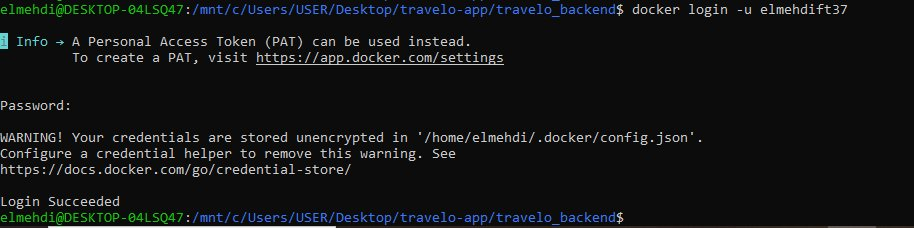
\includegraphics[width=0.95\textwidth]{./screenshots/volet1/10_connexion_docker_hub_reussie.png}
    \caption{Connexion Docker Hub réussie}
\end{figure}

\begin{figure}[H]
    \centering
    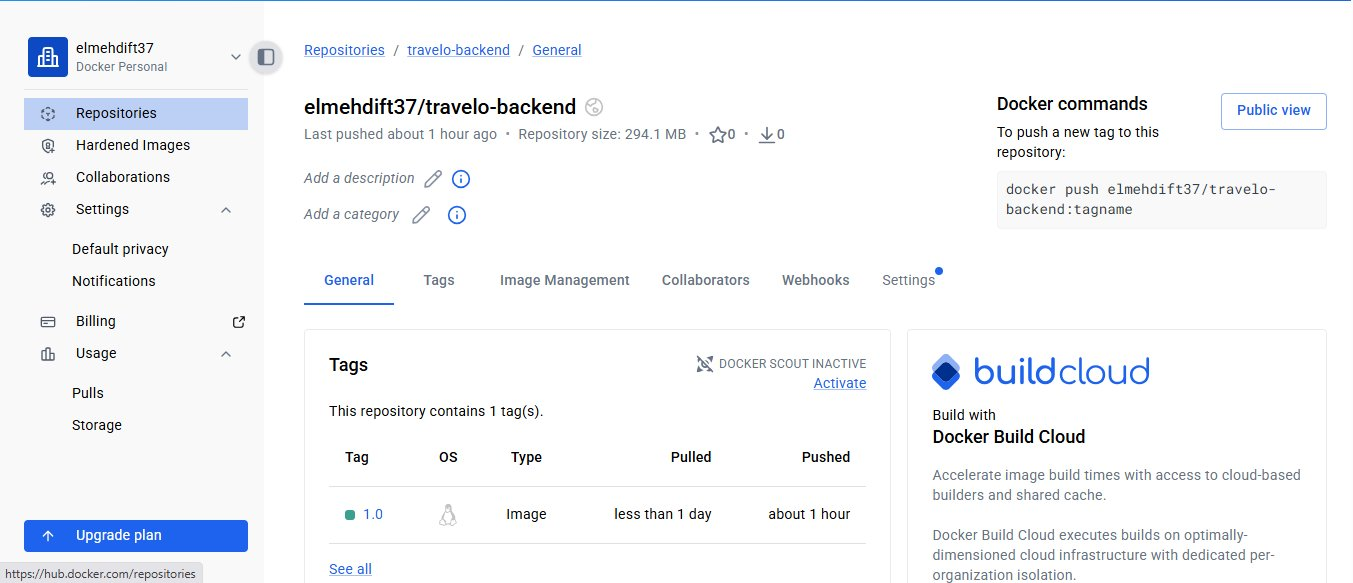
\includegraphics[width=0.95\textwidth]{./screenshots/volet1/11_push_travelo_backend_1.0_docker_hub.png}
    \caption{elmehdift37/travelo-backend:1.0 publié sur Docker Hub}
\end{figure}

\subsubsection{5.d. Lancement du conteneur Backend}

\begin{lstlisting}[language=bash]
docker run -d --name travelo-backend --network travelo-network -p 8080:8080 \
  -e SPRING_DATASOURCE_URL=jdbc:mysql://travelo_app:3306/travelo_db \
  -e SPRING_DATASOURCE_USERNAME=root -e SPRING_DATASOURCE_PASSWORD=password \
  elmehdift37/travelo-backend:1.0
\end{lstlisting}

\begin{figure}[H]
    \centering
    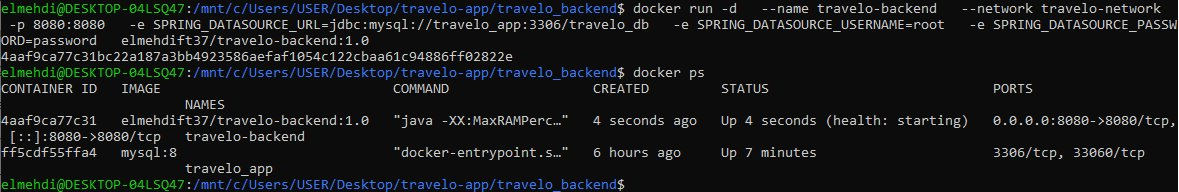
\includegraphics[width=0.95\textwidth]{./screenshots/volet1/12_conteneur_backend_demarre_docker_ps.png}
    \caption{Conteneur travelo-backend démarré (docker ps)}
\end{figure}

\begin{figure}[H]
    \centering
    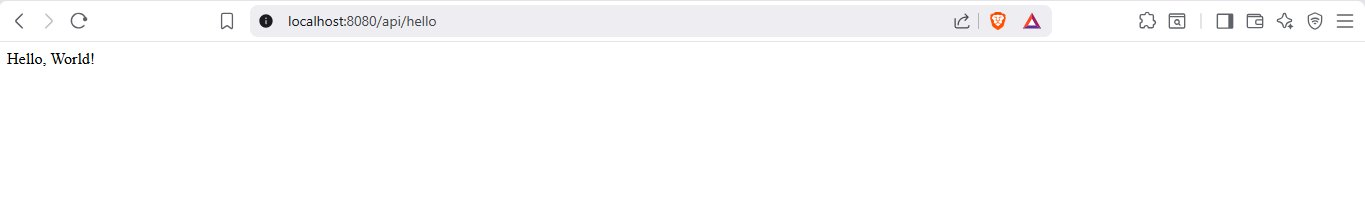
\includegraphics[width=0.95\textwidth]{./screenshots/volet1/13_api_backend_hello_world_localhost_8080.png}
    \caption{API Backend opérationnelle : "Hello, World!" sur localhost:8080/api/hello}
\end{figure}

\subsubsection{5.e. Inspection du conteneur Backend}

\begin{lstlisting}[language=bash]
docker inspect travelo-backend
\end{lstlisting}

\begin{figure}[H]
    \centering
    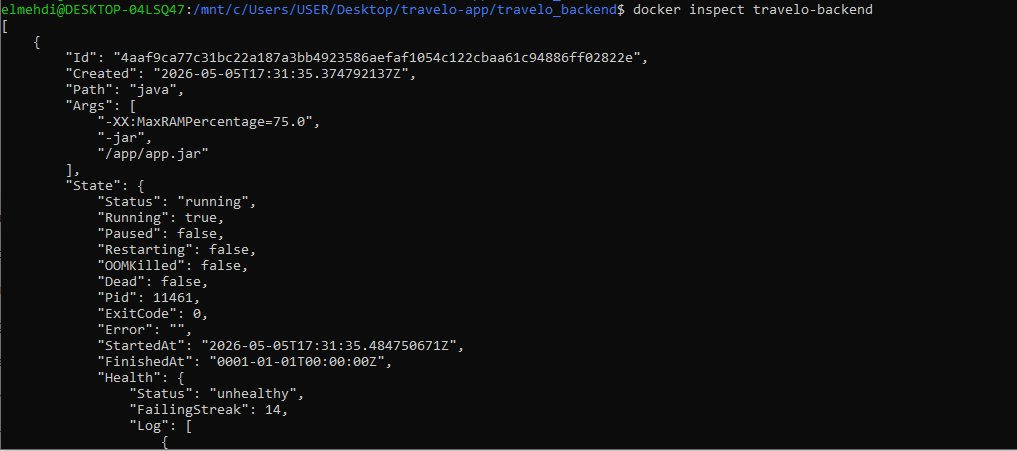
\includegraphics[width=0.95\textwidth]{./screenshots/volet1/14_docker_inspect_backend_running_healthcheck.png}
    \caption{\texttt{docker inspect travelo-backend} : état running, healthcheck configuré}
\end{figure}

\subsubsection{5.f. Logs du conteneur Backend}

\begin{lstlisting}[language=bash]
docker logs travelo-backend
\end{lstlisting}

\begin{figure}[H]
    \centering
    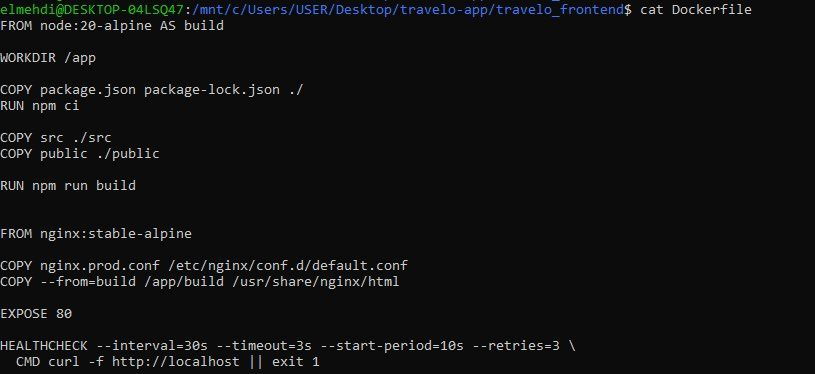
\includegraphics[width=0.95\textwidth]{./screenshots/volet1/15_logs_backend_spring_boot_v3.4.0_port_8080.png}
    \caption{Logs travelo-backend : Spring Boot v3.4.0 démarré sur port 8080}
\end{figure}



\subsection{6. Dockerfile Frontend \& Image}

\begin{figure}[H]
    \centering
    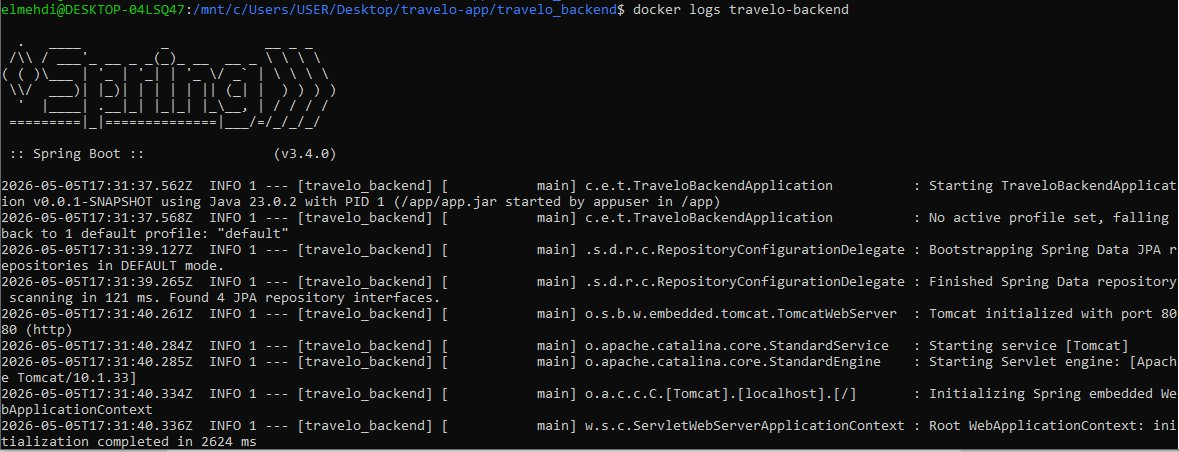
\includegraphics[width=0.95\textwidth]{./screenshots/volet1/16_dockerfile_frontend_node20_alpine_nginx_alpine.png}
    \caption{Dockerfile Frontend : Node:20-alpine (build) + nginx:stable-alpine (runtime)}
\end{figure}

\subsubsection{Bonnes pratiques Frontend}

\begin{itemize}
    \item Multi-stage build Node → Nginx Alpine (\textasciitilde{}95MB)
    \item \texttt{npm ci} pour builds reproductibles
    \item \texttt{package.json} copié séparément pour le cache
    \item HEALTHCHECK Nginx
    \item EXPOSE 80
\end{itemize}

\begin{lstlisting}[language=bash]
docker build -t travelo-frontend .
\end{lstlisting}

\begin{figure}[H]
    \centering
    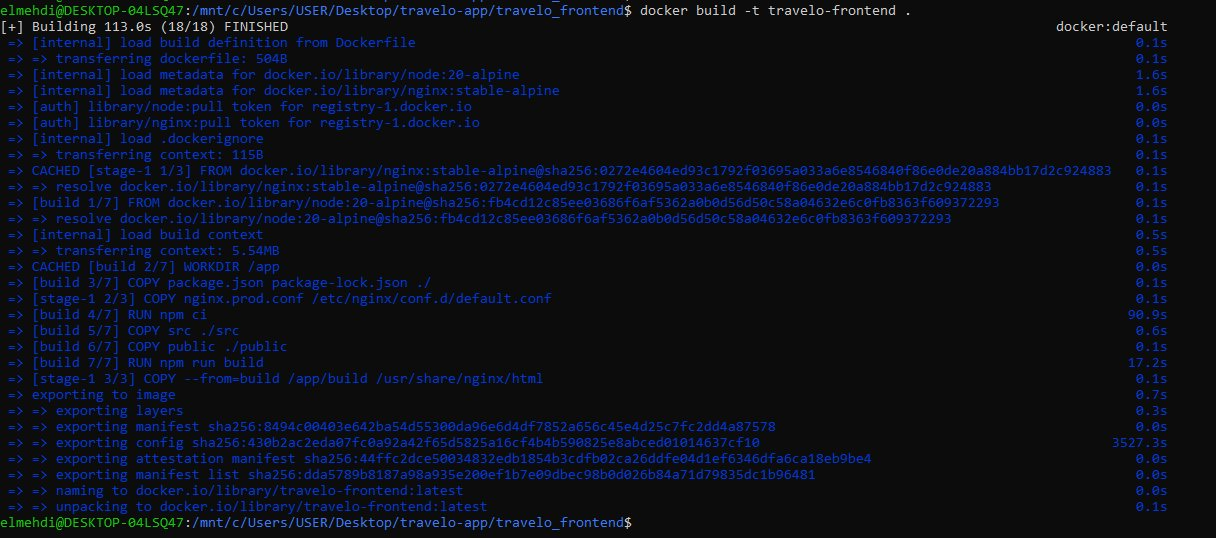
\includegraphics[width=0.95\textwidth]{./screenshots/volet1/17_build_frontend_travelo_succes_18_etapes_95MB.png}
    \caption{Build travelo-frontend réussi (18/18 étapes, 95.2MB)}
\end{figure}

\begin{figure}[H]
    \centering
    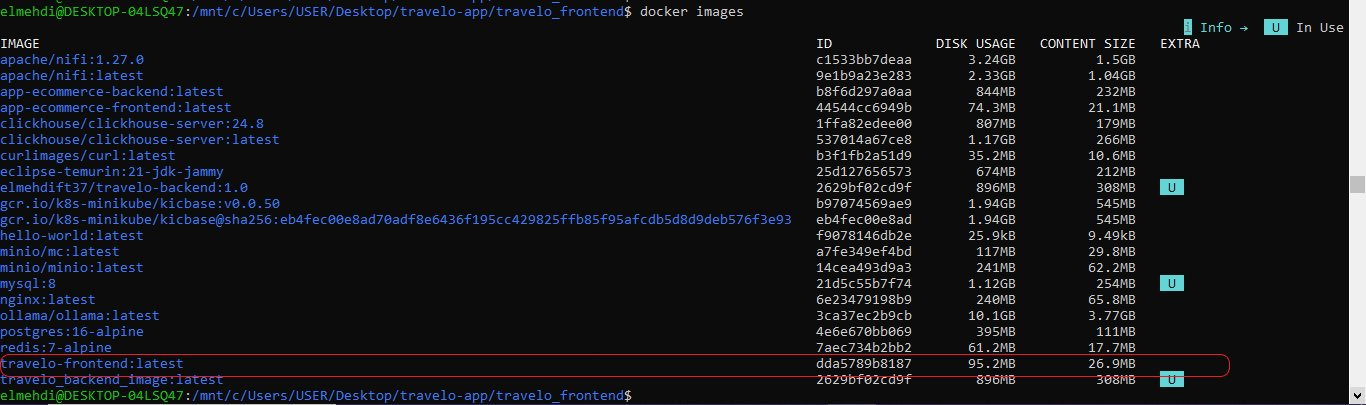
\includegraphics[width=0.95\textwidth]{./screenshots/volet1/18_docker_images_travelo_frontend_et_backend.png}
    \caption{\texttt{docker images} : travelo-frontend:latest et travelo\_backend\_image:latest}
\end{figure}

\subsubsection{Scan Trivy Frontend}

\begin{lstlisting}[language=bash]
trivy image travelo-frontend
\end{lstlisting}

3 vulnérabilités (2 MEDIUM, 1 HIGH) sur Alpine 3.23.4 : libxpm, nghttp2-libs, xz-libs. Toutes disposent de versions corrigées disponibles via mise à jour de l'image de base.

\begin{figure}[H]
    \centering
    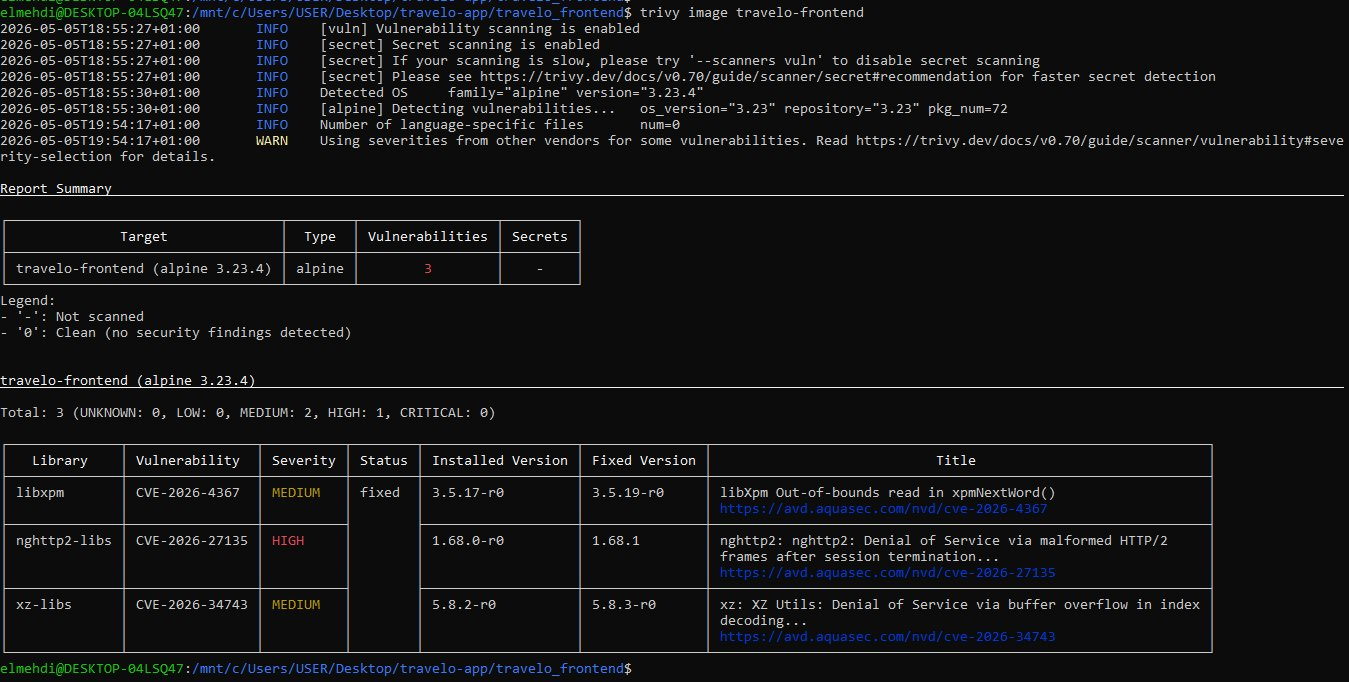
\includegraphics[width=0.95\textwidth]{./screenshots/volet1/19_trivy_scan_frontend_3_vulnerabilites_alpine.png}
    \caption{Trivy frontend : 3 vulnérabilités (libxpm, nghttp2-libs, xz-libs)}
\end{figure}

\subsubsection{Publication Frontend sur Docker Hub}

\begin{lstlisting}[language=bash]
docker tag travelo-frontend elmehdift37/travelo-frontend:1.0
docker push elmehdift37/travelo-frontend:1.0
\end{lstlisting}

\begin{figure}[H]
    \centering
    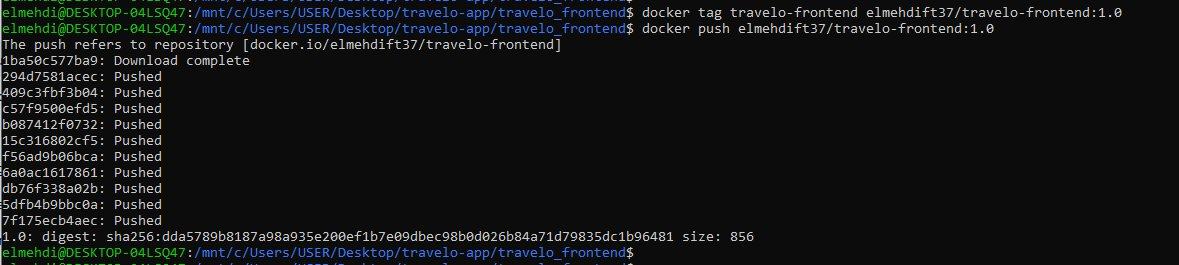
\includegraphics[width=0.95\textwidth]{./screenshots/volet1/20_push_travelo_frontend_1.0_docker_hub.png}
    \caption{Push travelo-frontend:1.0 vers Docker Hub}
\end{figure}

\begin{figure}[H]
    \centering
    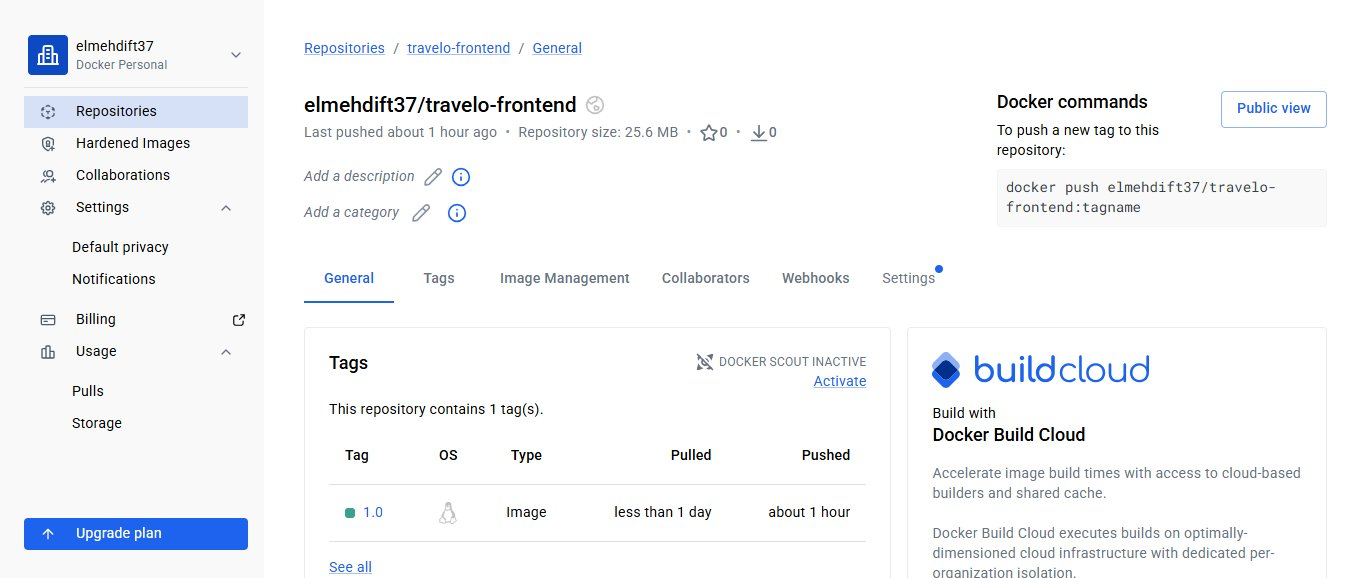
\includegraphics[width=0.95\textwidth]{./screenshots/volet1/21_docker_hub_travelo_frontend_tag_1.0_25MB.png}
    \caption{elmehdift37/travelo-frontend sur Docker Hub (tag 1.0, 25.6MB)}
\end{figure}

\subsubsection{Lancement du conteneur Frontend}

\begin{lstlisting}[language=bash]
docker run -d --name travelo-frontend --network travelo-network -p 3000:80 elmehdift37/travelo-frontend:1.0
\end{lstlisting}

\begin{figure}[H]
    \centering
    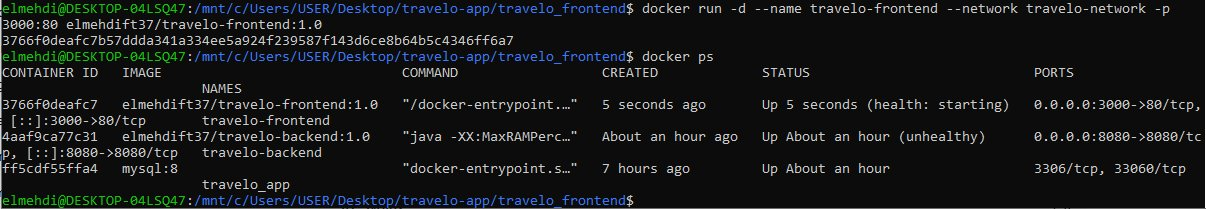
\includegraphics[width=0.95\textwidth]{./screenshots/volet1/22_docker_ps_3_conteneurs_mysql_backend_frontend_actifs.png}
    \caption{Les 3 conteneurs actifs : mysql, travelo-backend, travelo-frontend}
\end{figure}



\subsection{7. Vérification du bon fonctionnement de l'application}

Les trois conteneurs étant démarrés, l'application Travelo est accessible depuis le navigateur sur localhost:3000.

\begin{figure}[H]
    \centering
    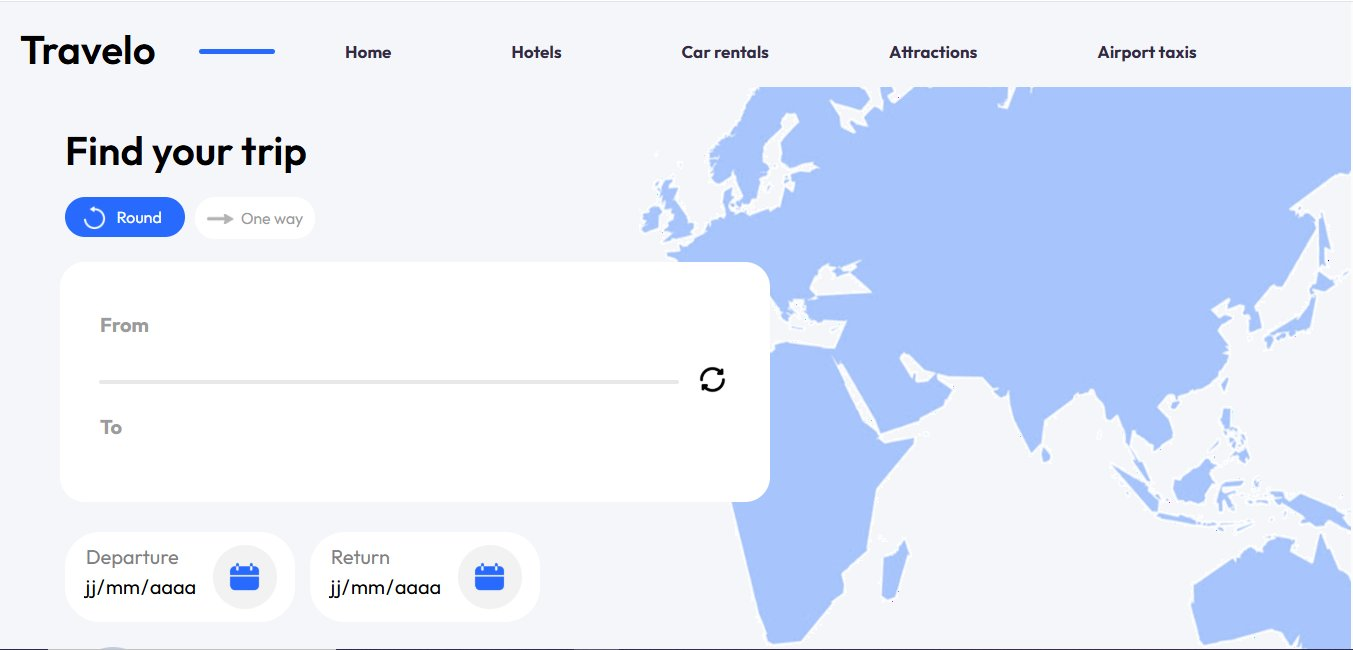
\includegraphics[width=0.95\textwidth]{./screenshots/volet1/23_interface_travelo_localhost_3000_find_your_trip.png}
    \caption{Interface Travelo sur localhost:3000 : page "Find your trip"}
\end{figure}

\subsubsection{Inspection du Frontend}

\begin{lstlisting}[language=bash]
docker inspect travelo-frontend
\end{lstlisting}

\begin{figure}[H]
    \centering
    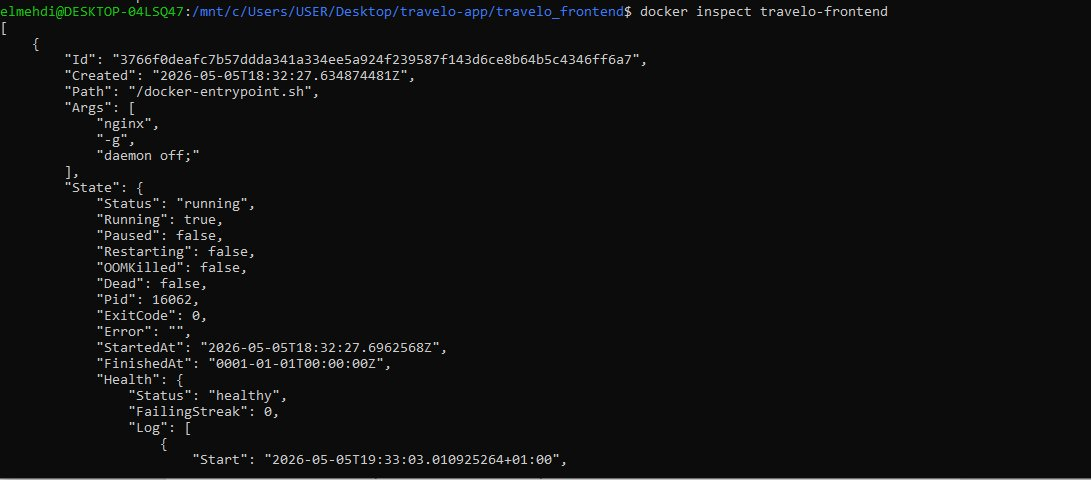
\includegraphics[width=0.95\textwidth]{./screenshots/volet1/24_docker_inspect_frontend_running_healthy.png}
    \caption{\texttt{docker inspect travelo-frontend} : état running, health: healthy}
\end{figure}

\subsubsection{Logs du Frontend}

\begin{lstlisting}[language=bash]
docker logs travelo-frontend
\end{lstlisting}

\begin{figure}[H]
    \centering
    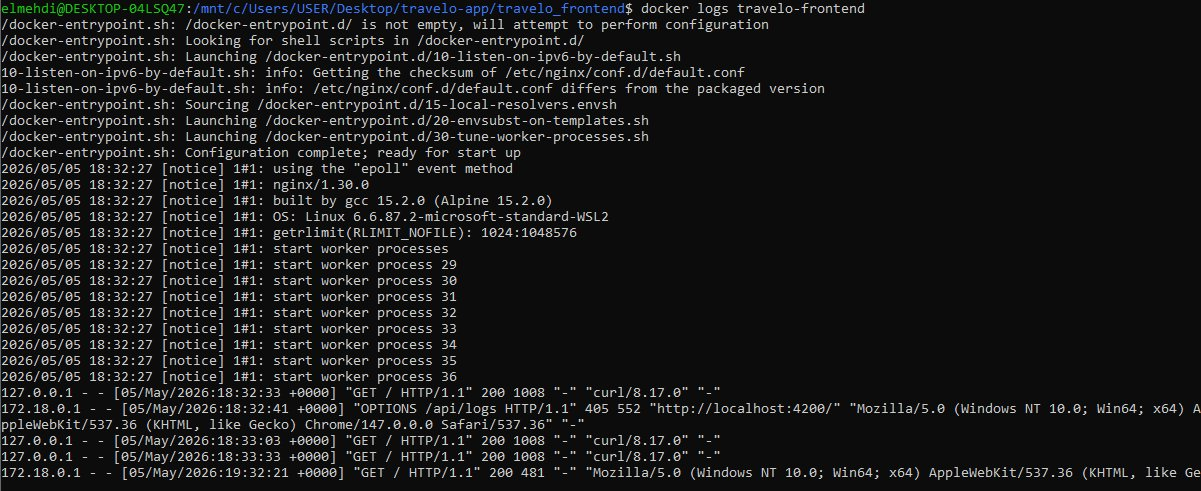
\includegraphics[width=0.95\textwidth]{./screenshots/volet1/25_logs_nginx_1.30.0_demarrage_requetes_http.png}
    \caption{Logs Nginx 1.30.0 : démarrage et requêtes HTTP traitées}
\end{figure}

\subsubsection{Test fonctionnel – Formulaire de réservation}

\begin{figure}[H]
    \centering
    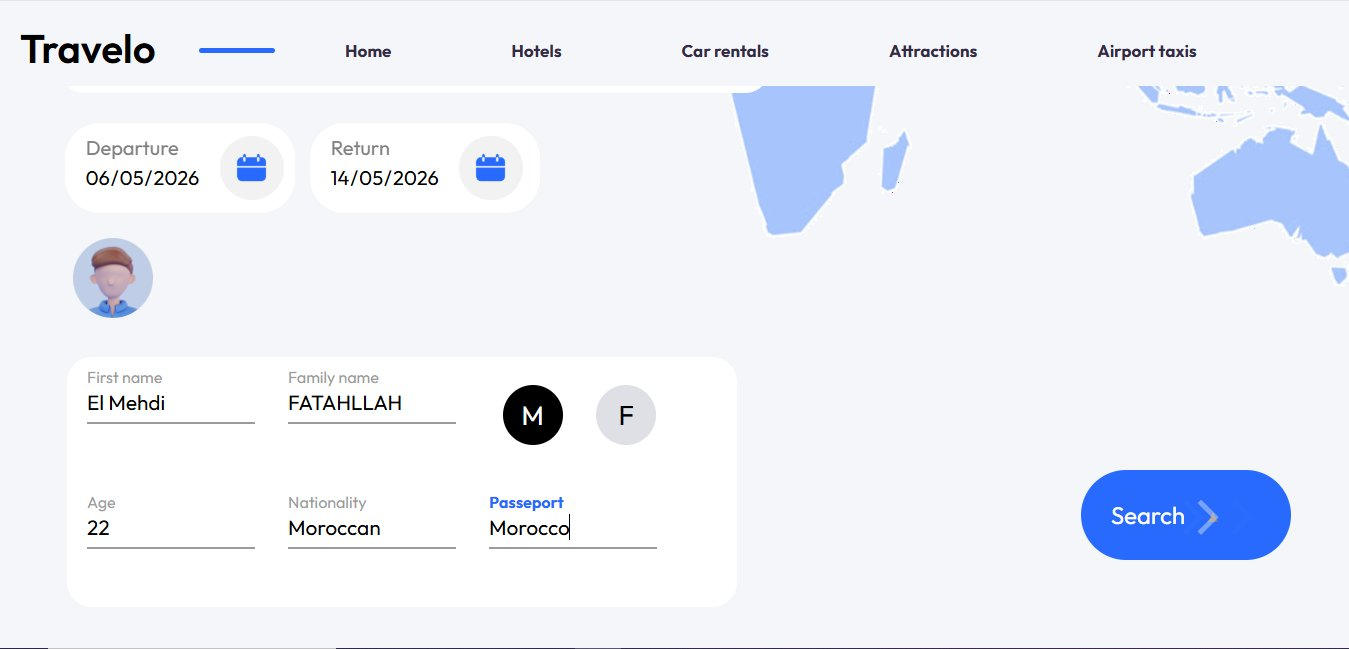
\includegraphics[width=0.95\textwidth]{./screenshots/volet1/26_formulaire_passager_elmehdi_fatahllah_moroccan.png}
    \caption{Formulaire passager renseigné (El Mehdi FATAHLLAH, Moroccan)}
\end{figure}



\subsection{8. Suppression des conteneurs}

\begin{lstlisting}[language=bash]
docker rm -f travelo-backend travelo-frontend travelo_app
\end{lstlisting}

\begin{itemize}
    \item \texttt{docker rm -f} : Suppression forcée des conteneurs, même en cours d'exécution
\end{itemize}

\begin{figure}[H]
    \centering
    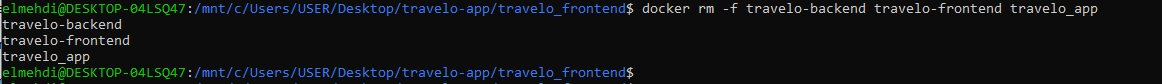
\includegraphics[width=0.95\textwidth]{./screenshots/volet1/27_suppression_forcee_3_conteneurs_docker_rm.png}
    \caption{Suppression forcée des 3 conteneurs}
\end{figure}

\begin{figure}[H]
    \centering
    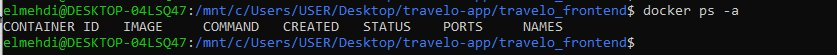
\includegraphics[width=0.95\textwidth]{./screenshots/volet1/28_docker_ps_aucun_conteneur_restant.png}
    \caption{\texttt{docker ps -a} : aucun conteneur actif restant}
\end{figure}



\subsection{9. Redéploiement avec Docker Compose}

\subsubsection{9.a. Fichier docker-compose.yml}

\begin{figure}[H]
    \centering
    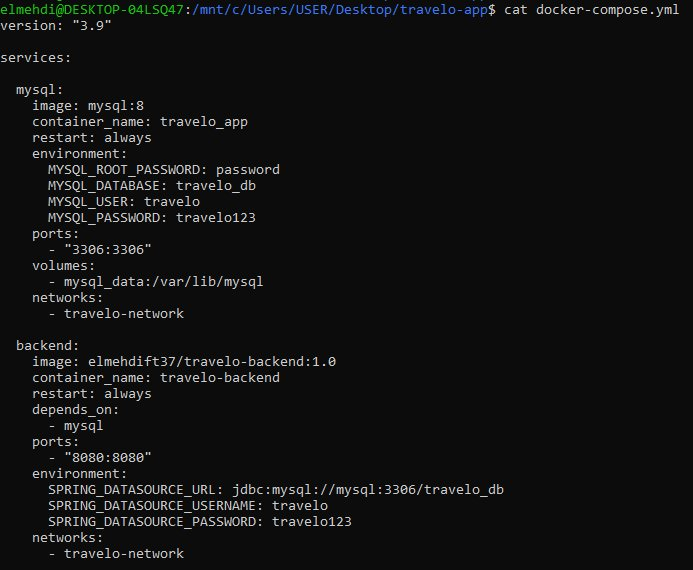
\includegraphics[width=0.95\textwidth]{./screenshots/volet1/29_docker_compose_yml_services_mysql_backend.png}
    \caption{docker-compose.yml : services mysql et backend}
\end{figure}

\begin{figure}[H]
    \centering
    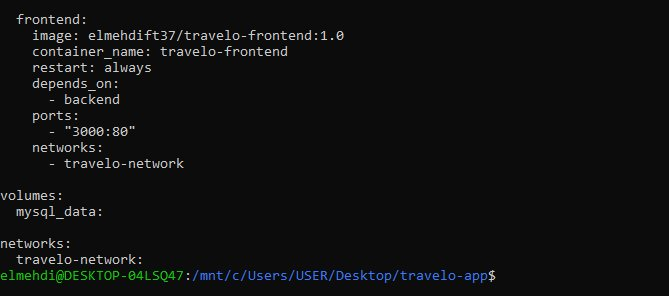
\includegraphics[width=0.95\textwidth]{./screenshots/volet1/30_docker_compose_yml_service_frontend_volumes_reseau.png}
    \caption{docker-compose.yml : service frontend, volumes et réseau}
\end{figure}

Points clés : \texttt{depends\_on} (ordre de démarrage), \texttt{restart: always}, réseau commun \texttt{travelo-network}, volume \texttt{mysql\_data} persistant.

\subsubsection{9.b. Lancement}

\begin{lstlisting}[language=bash]
docker compose up -d
\end{lstlisting}

\begin{figure}[H]
    \centering
    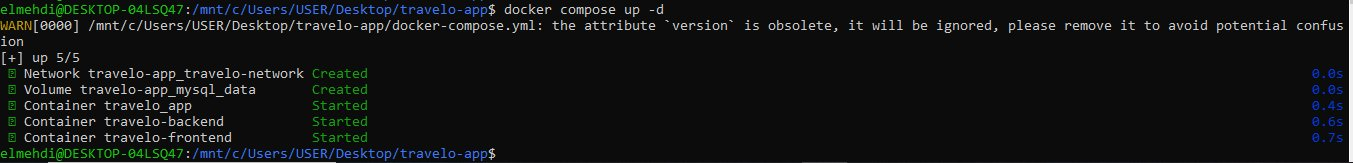
\includegraphics[width=0.95\textwidth]{./screenshots/volet1/31_docker_compose_up_reseau_volume_3_conteneurs_crees.png}
    \caption{docker compose up -d : réseau, volume et 3 conteneurs créés}
\end{figure}

\begin{figure}[H]
    \centering
    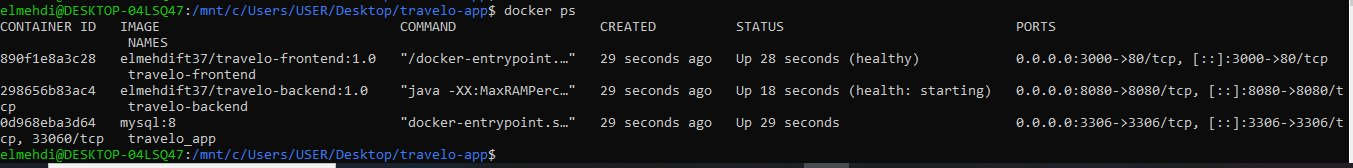
\includegraphics[width=0.95\textwidth]{./screenshots/volet1/32_docker_ps_3_conteneurs_up_avec_ports.png}
    \caption{\texttt{docker ps} : les 3 conteneurs "Up" avec leurs ports}
\end{figure}

\subsubsection{9.c. Vérification}

\begin{figure}[H]
    \centering
    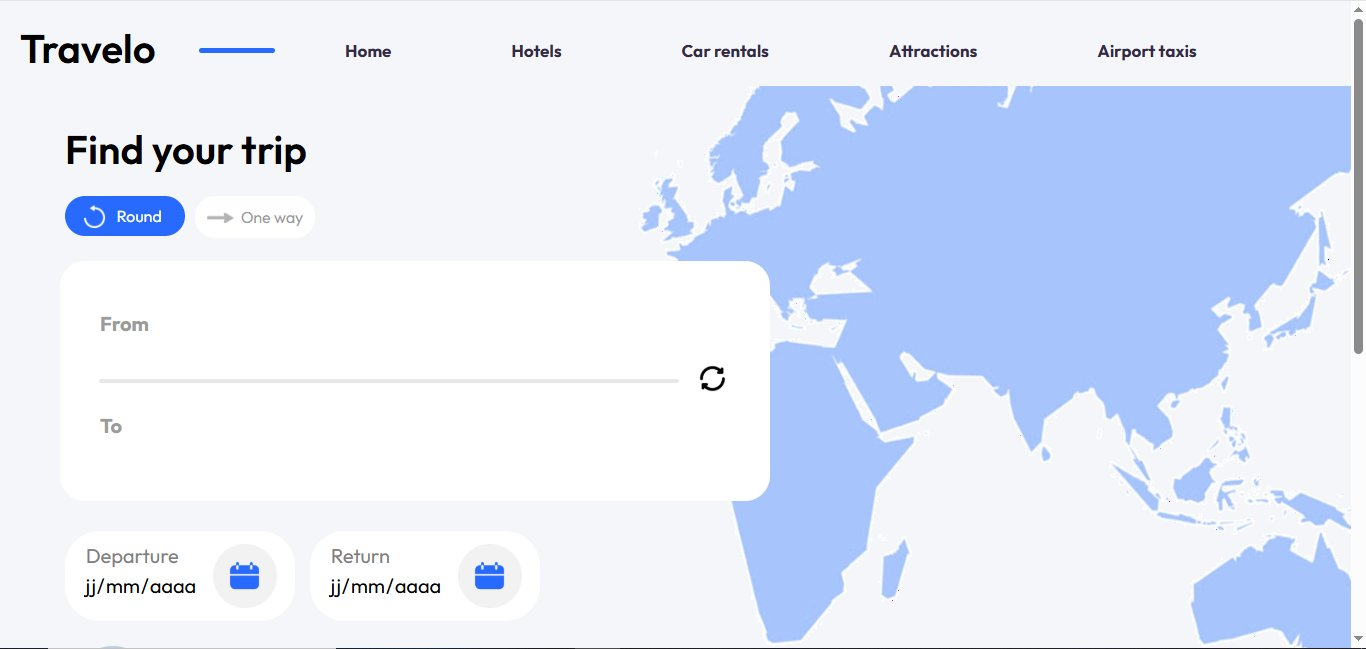
\includegraphics[width=0.95\textwidth]{./screenshots/volet1/33_travelo_fonctionnel_docker_compose_localhost_3000.png}
    \caption{Application Travelo fonctionnelle via Docker Compose (localhost:3000)}
\end{figure}



\subsection{10. Suppression des conteneurs et images}

\begin{lstlisting}[language=bash]
docker rm -f travelo-backend travelo-frontend travelo_app
docker rmi -f elmehdift37/travelo-frontend:1.0 elmehdift37/travelo-backend:1.0 mysql:8
\end{lstlisting}

\begin{figure}[H]
    \centering
    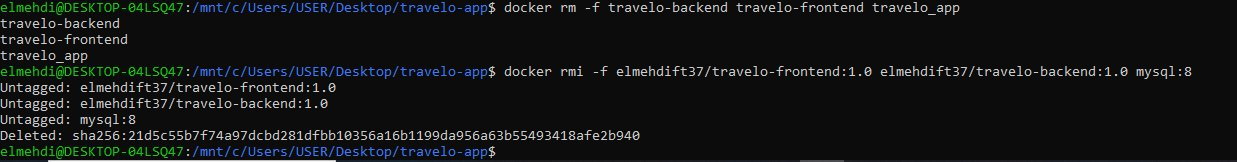
\includegraphics[width=0.95\textwidth]{./screenshots/volet1/34_suppression_conteneurs_et_images_docker_locales.png}
    \caption{Suppression des conteneurs et des images Docker locales}
\end{figure}



\subsection{11. Registre privé local d'images Docker}

Un registre privé Docker est déployé localement via deux services : \texttt{registry:2} (port 5000) pour le stockage, et \texttt{joxit/docker-registry-ui} (port 8081) pour la visualisation via navigateur.

\subsubsection{Fichier docker-compose.yml du registre}

\begin{figure}[H]
    \centering
    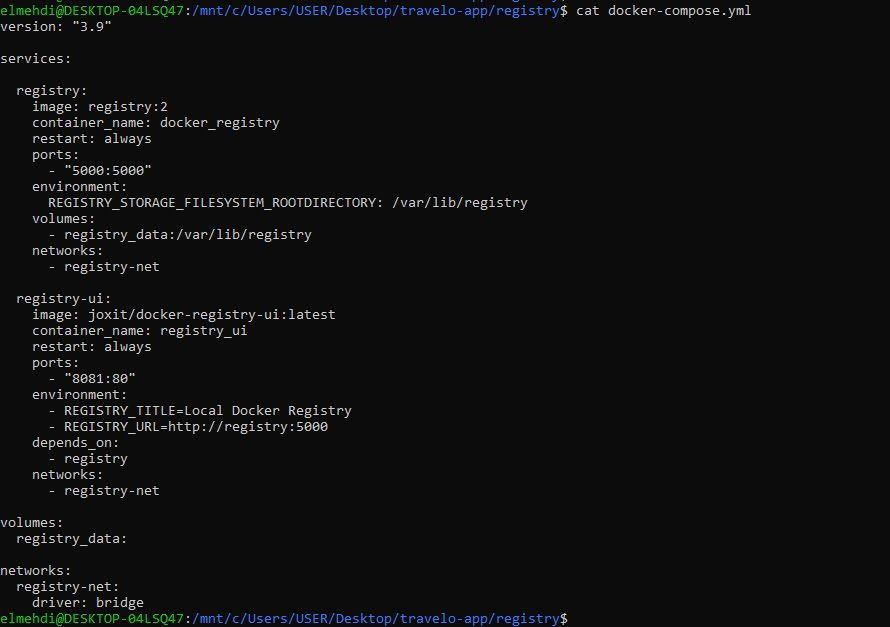
\includegraphics[width=0.95\textwidth]{./screenshots/volet1/35_docker_compose_yml_registre_prive_registry2_ui.png}
    \caption{docker-compose.yml du registre privé (registry:2 + docker-registry-ui)}
\end{figure}

\subsubsection{Démarrage du registre}

\begin{lstlisting}[language=bash]
docker compose up -d
\end{lstlisting}

\begin{figure}[H]
    \centering
    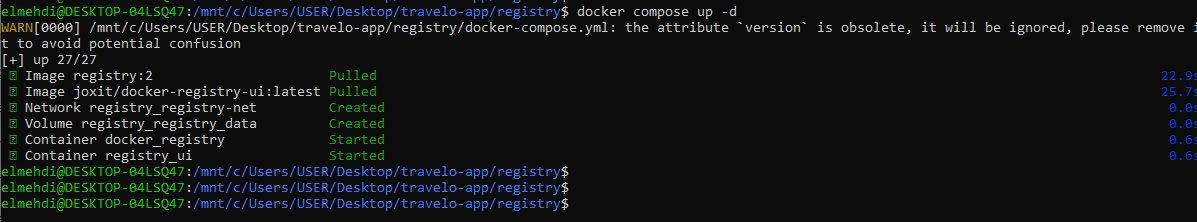
\includegraphics[width=0.95\textwidth]{./screenshots/volet1/36_demarrage_registre_docker_registry_port5000_ui_port8081.png}
    \caption{Démarrage du registre : docker\_registry (port 5000) et registry\_ui (port 8081)}
\end{figure}

\begin{figure}[H]
    \centering
    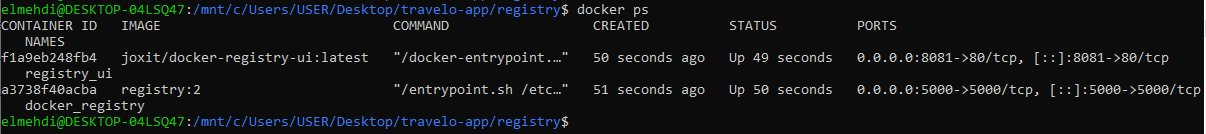
\includegraphics[width=0.95\textwidth]{./screenshots/volet1/37_docker_ps_registry2_et_registry_ui_actifs.png}
    \caption{\texttt{docker ps} : registry:2 et registry\_ui actifs}
\end{figure}

\subsubsection{Push des images vers le registre privé}

\begin{lstlisting}[language=bash]
docker tag travelo-frontend localhost:5000/travelo-frontend:1.0
docker push localhost:5000/travelo-frontend:1.0
docker tag elmehdift37/travelo-backend:1.0 localhost:5000/travelo-backend:1.0
docker push localhost:5000/travelo-backend:1.0
\end{lstlisting}

\begin{figure}[H]
    \centering
    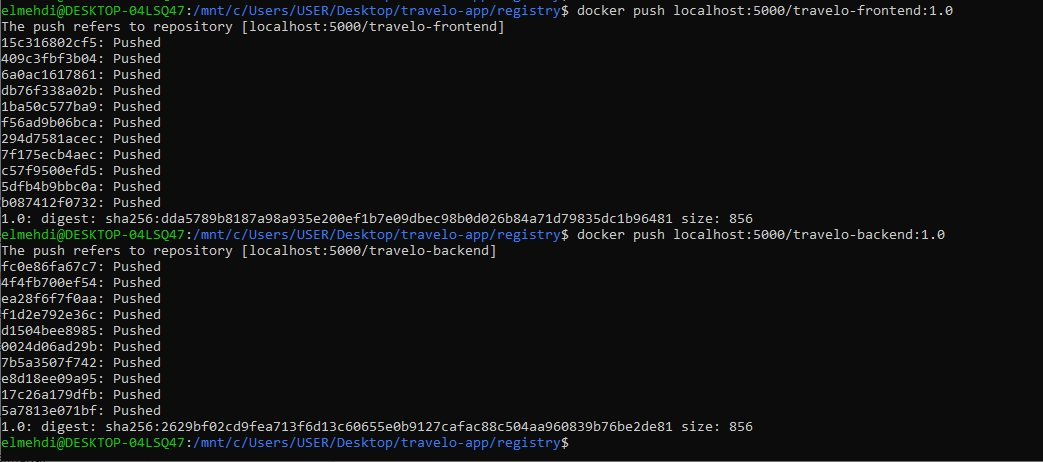
\includegraphics[width=0.95\textwidth]{./screenshots/volet1/38_push_images_vers_localhost_5000_backend_frontend.png}
    \caption{Push des deux images vers localhost:5000}
\end{figure}

\subsubsection{Visualisation via l'interface UI}

\begin{figure}[H]
    \centering
    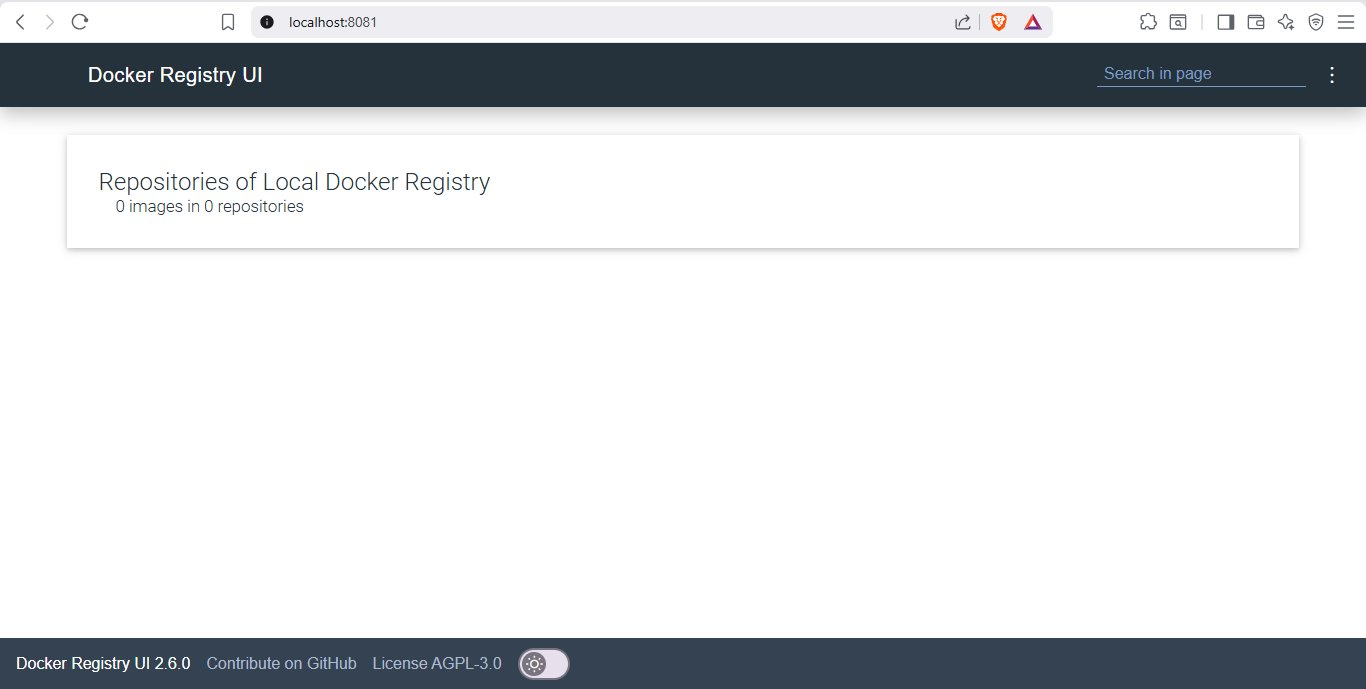
\includegraphics[width=0.95\textwidth]{./screenshots/volet1/39_docker_registry_ui_vide_localhost_8081.png}
    \caption{Docker Registry UI vide au démarrage (localhost:8081)}
\end{figure}

\begin{figure}[H]
    \centering
    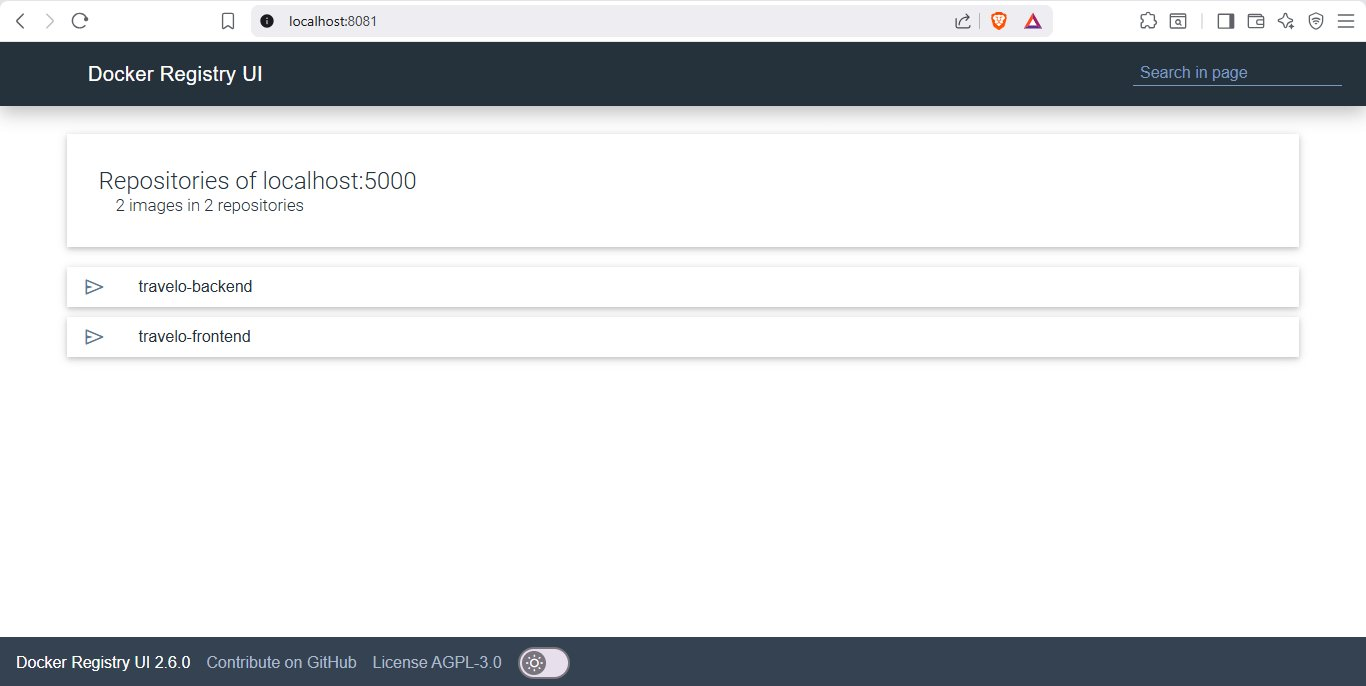
\includegraphics[width=0.95\textwidth]{./screenshots/volet1/40_docker_registry_ui_2_depots_backend_frontend.png}
    \caption{Docker Registry UI : 2 images dans 2 dépôts (travelo-backend, travelo-frontend)}
\end{figure}

\begin{figure}[H]
    \centering
    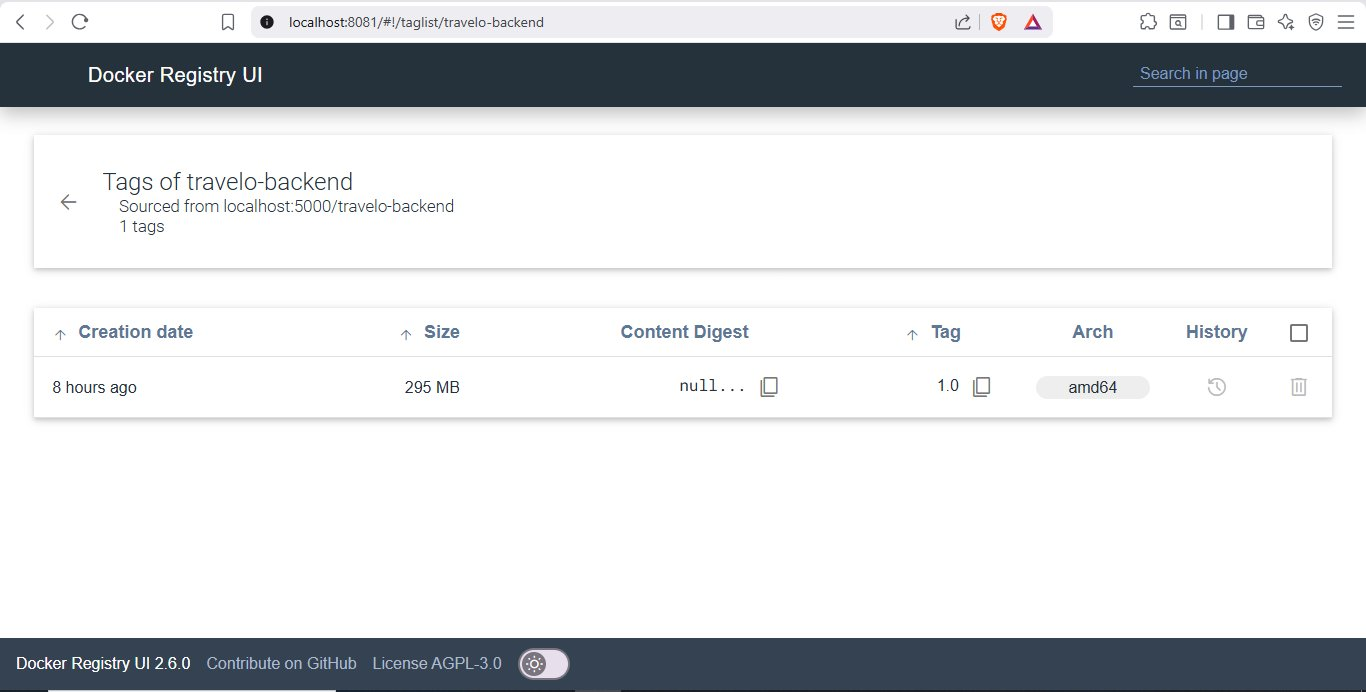
\includegraphics[width=0.95\textwidth]{./screenshots/volet1/41_detail_depot_travelo_backend_tag1.0_295MB_amd64.png}
    \caption{Détail du dépôt travelo-backend : tag 1.0, 295MB, architecture amd64}
\end{figure}

\begin{figure}[H]
    \centering
    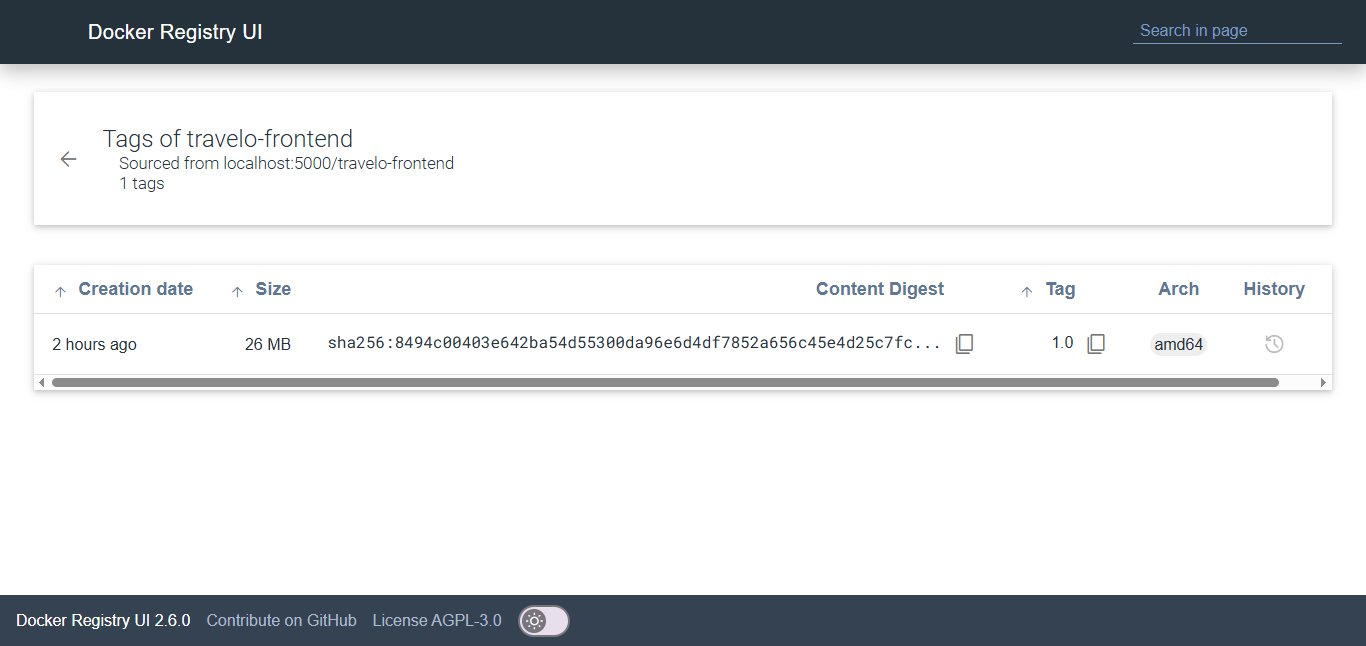
\includegraphics[width=0.95\textwidth]{./screenshots/volet1/42_detail_depot_travelo_frontend_tag1.0_digest_sha256.png}
    \caption{Détail du dépôt travelo-frontend : tag 1.0, digest SHA256 visible}
\end{figure}



\subsection{12. Redéploiement depuis le registre privé}

Un nouveau fichier docker-compose.yml est créé en remplaçant les références Docker Hub par \texttt{localhost:5000} pour utiliser les images du registre privé local.

\subsubsection{Fichier docker-compose.yml avec registre privé}

\begin{figure}[H]
    \centering
    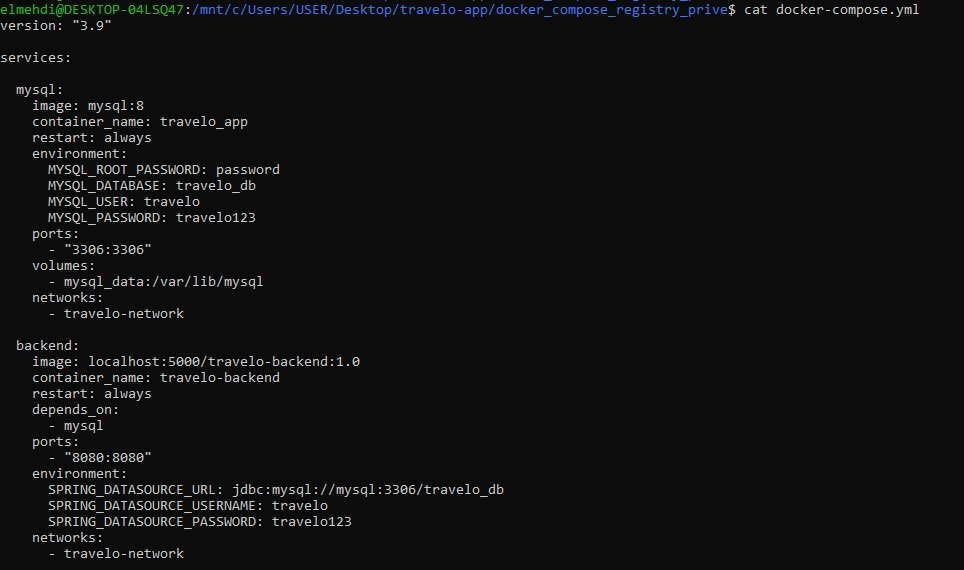
\includegraphics[width=0.95\textwidth]{./screenshots/volet1/43_docker_compose_yml_images_registre_prive_localhost_5000.png}
    \caption{docker-compose.yml avec image: localhost:5000/travelo-backend:1.0 et localhost:5000/travelo-frontend:1.0}
\end{figure}

\begin{figure}[H]
    \centering
    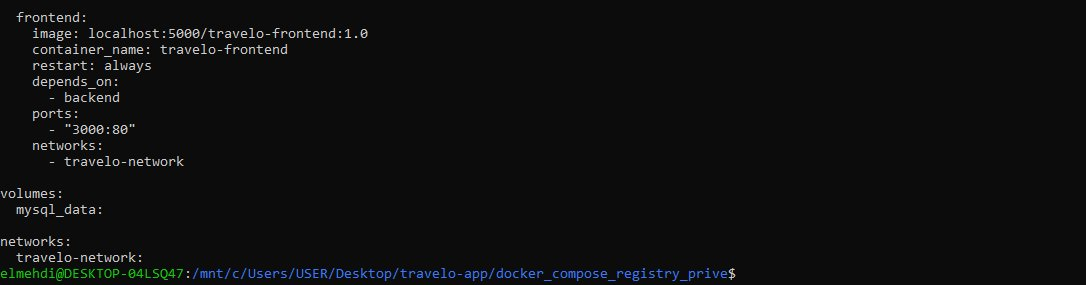
\includegraphics[width=0.95\textwidth]{./screenshots/volet1/44_docker_compose_yml_service_frontend_registre_local_port3000.png}
    \caption{Suite du docker-compose.yml : service frontend depuis le registre local (port 3000)}
\end{figure}

\subsubsection{Démarrage depuis le registre privé}

\begin{lstlisting}[language=bash]
docker compose up -d
\end{lstlisting}

\begin{figure}[H]
    \centering
    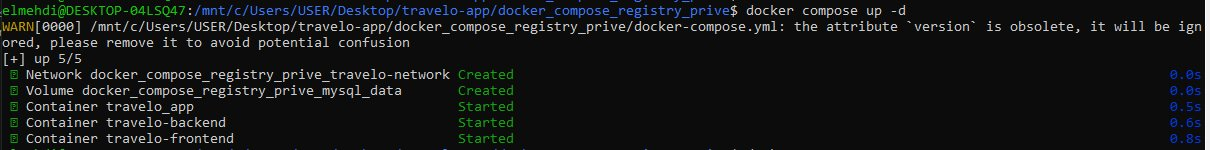
\includegraphics[width=0.95\textwidth]{./screenshots/volet1/45_docker_compose_up_3_conteneurs_depuis_localhost_5000.png}
    \caption{docker compose up -d : réseau, volume et 3 conteneurs démarrés depuis localhost:5000}
\end{figure}

\begin{figure}[H]
    \centering
    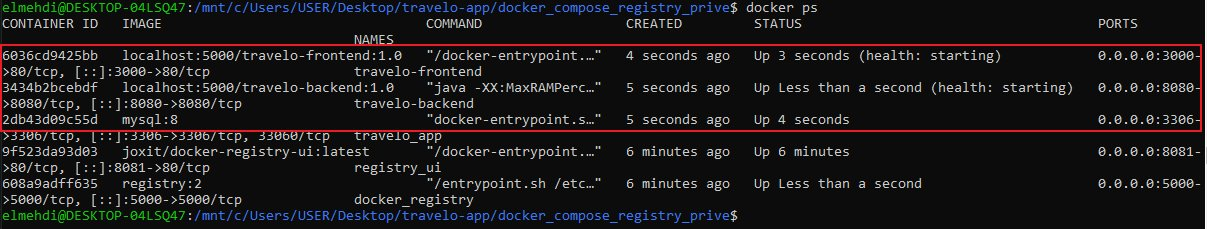
\includegraphics[width=0.95\textwidth]{./screenshots/volet1/46_docker_ps_frontend_backend_depuis_localhost_5000_actifs.png}
    \caption{\texttt{docker ps} : travelo-frontend et travelo-backend tirés depuis localhost:5000, tous actifs}
\end{figure}

\subsubsection{Vérification de l'application}

\begin{figure}[H]
    \centering
    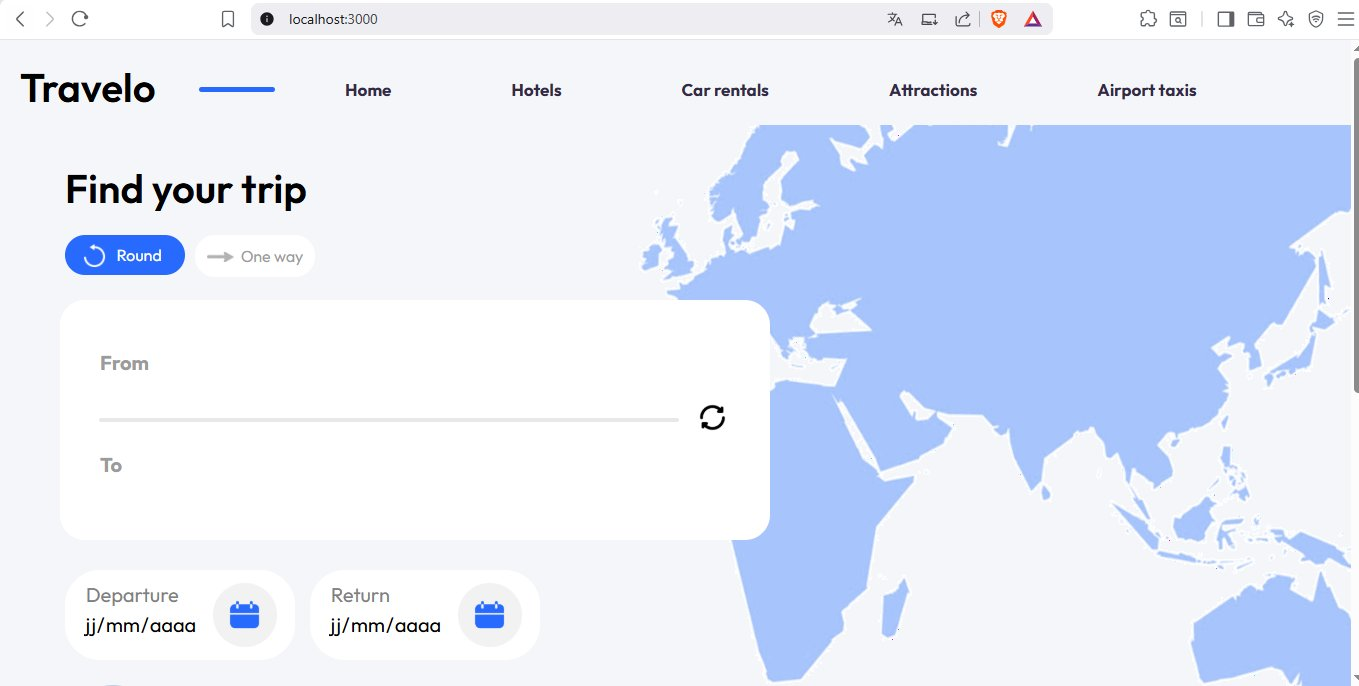
\includegraphics[width=0.95\textwidth]{./screenshots/volet1/47_travelo_fonctionnel_depuis_registre_prive_localhost_3000.png}
    \caption{Application Travelo fonctionnelle depuis le registre privé (localhost:3000)}
\end{figure}



\subsection{Bonus : Déploiement Docker Swarm}

Docker Swarm est un orchestrateur natif de Docker permettant de gérer un cluster de nœuds, d'assurer la haute disponibilité par réplication des services, et d'équilibrer automatiquement la charge.

\subsubsection{Fichier docker-compose.yml compatible Swarm}

Le fichier de stack Swarm définit 4 services : mysql (1 réplica, manager), backend (2 réplicas), frontend (2 réplicas), et traefik (reverse proxy). Chaque service dispose d'une politique de redémarrage et de limites de ressources CPU/mémoire.

\begin{figure}[H]
    \centering
    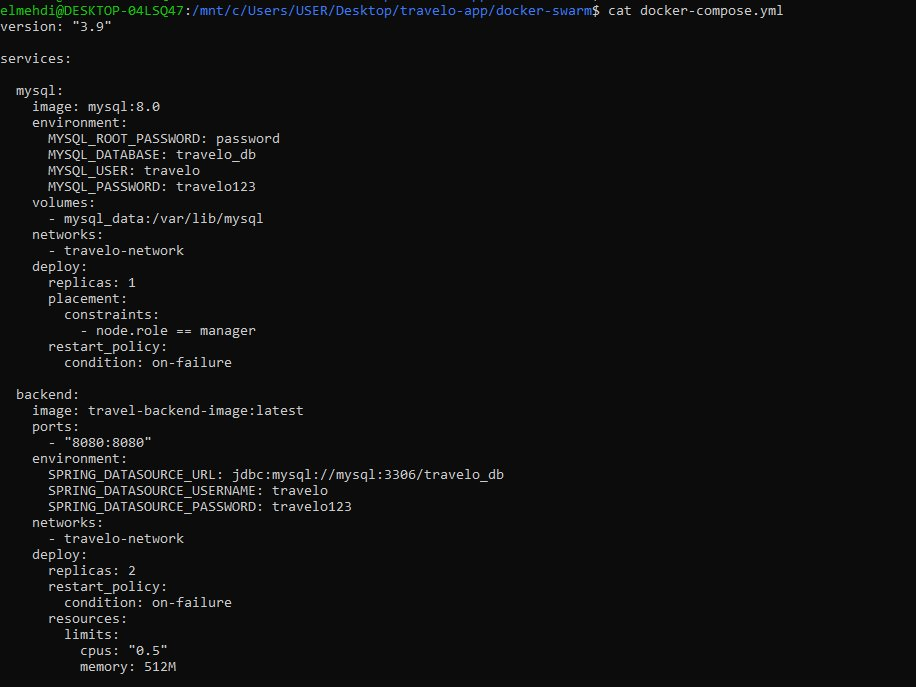
\includegraphics[width=0.95\textwidth]{./screenshots/volet1/48_docker_compose_swarm_services_mysql_backend_replicas.png}
    \caption{docker-compose.yml Swarm : services mysql et backend (réplicas, restart\_policy, resource limits)}
\end{figure}

\begin{figure}[H]
    \centering
    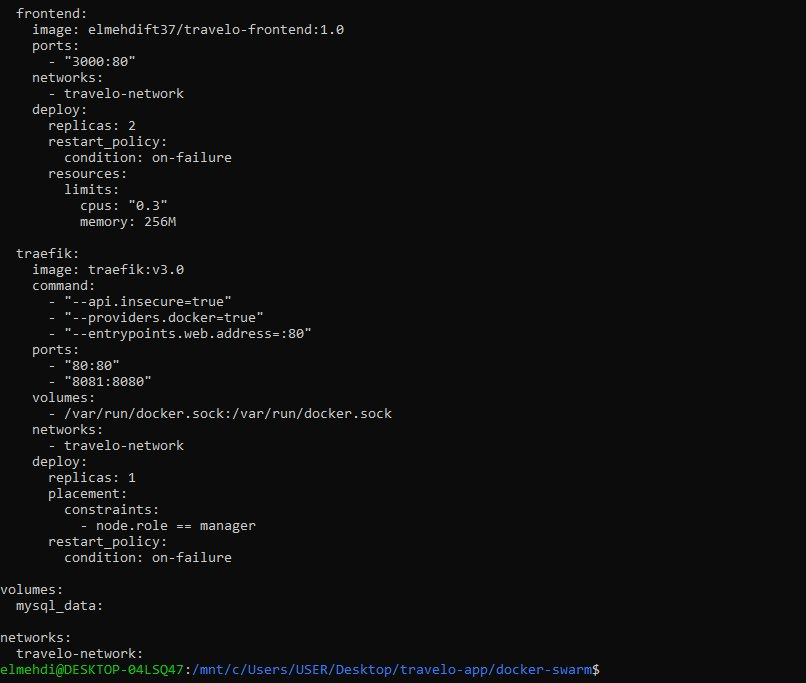
\includegraphics[width=0.95\textwidth]{./screenshots/volet1/49_docker_compose_swarm_service_frontend_2_replicas_traefik.png}
    \caption{docker-compose.yml Swarm : service frontend (2 réplicas, 0.3 CPU, 256M) + Traefik (reverse proxy)}
\end{figure}



\subsection{13. Initialisation du cluster Docker Swarm}

La commande \texttt{docker swarm init} initialise le nœud courant comme manager du cluster. Un token de jonction est généré pour l'ajout de workers.

\begin{lstlisting}[language=bash]
docker swarm init
\end{lstlisting}

\begin{figure}[H]
    \centering
    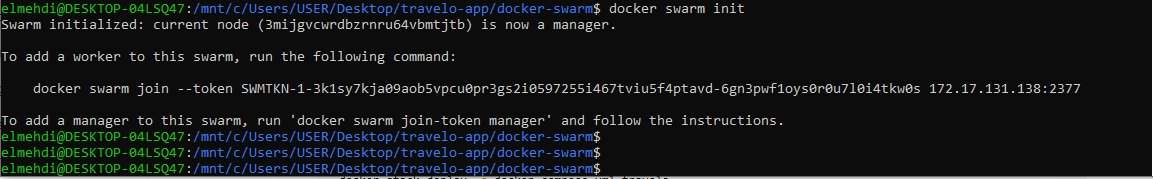
\includegraphics[width=0.95\textwidth]{./screenshots/volet1/50_docker_swarm_init_noeud_manager_leader.png}
    \caption{docker swarm init : nœud DESKTOP-04LSQ47 initialisé comme manager (Leader)}
\end{figure}

\subsubsection{Vérification des nœuds}

\begin{lstlisting}[language=bash]
docker node ls
\end{lstlisting}

\begin{figure}[H]
    \centering
    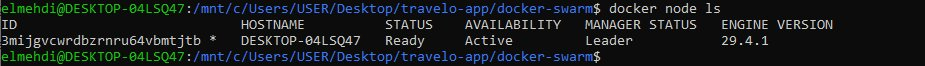
\includegraphics[width=0.95\textwidth]{./screenshots/volet1/51_docker_node_ls_1_noeud_manager_ready_leader.png}
    \caption{\texttt{docker node ls} : 1 nœud manager actif (Status: Ready, Manager Status: Leader)}
\end{figure}



\subsection{14 \& 15. Déploiement de la stack avec réplicas et limites de ressources}

La stack est déployée via \texttt{docker stack deploy} en utilisant le fichier docker-compose.yml. Chaque service est créé avec ses réplicas et ses contraintes de ressources définies dans la section \texttt{deploy}.

\begin{lstlisting}[language=bash]
docker stack deploy -c docker-compose.yml travelo_swarm
\end{lstlisting}

\begin{figure}[H]
    \centering
    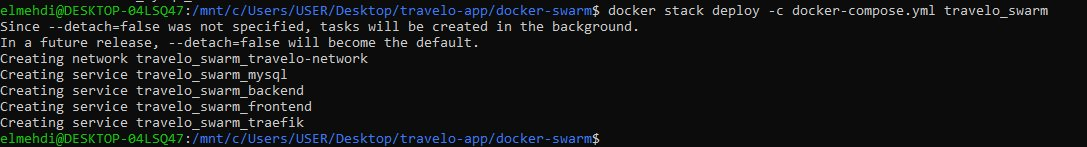
\includegraphics[width=0.95\textwidth]{./screenshots/volet1/52_stack_travelo_swarm_creation_reseau_4_services.png}
    \caption{Création de la stack travelo\_swarm : réseau + 4 services (mysql, backend, frontend, traefik)}
\end{figure}

\subsubsection{Vérification de la stack}

\begin{lstlisting}[language=bash]
docker stack ls
\end{lstlisting}

\begin{figure}[H]
    \centering
    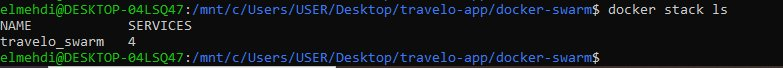
\includegraphics[width=0.95\textwidth]{./screenshots/volet1/53_docker_stack_ls_travelo_swarm_4_services.png}
    \caption{\texttt{docker stack ls} : stack travelo\_swarm avec 4 services}
\end{figure}

\subsubsection{Liste des services déployés}

\begin{lstlisting}[language=bash]
docker service ls
\end{lstlisting}

\begin{figure}[H]
    \centering
    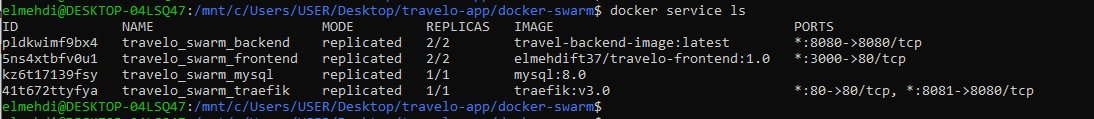
\includegraphics[width=0.95\textwidth]{./screenshots/volet1/54_docker_service_ls_backend_frontend_mysql_traefik_replicas.png}
    \caption{\texttt{docker service ls} : backend (2/2 réplicas), frontend (2/2), mysql (1/1), traefik (1/1)}
\end{figure}



\subsection{16. Restart Policy}

La politique de redémarrage \texttt{condition: on-failure} est configurée pour chaque service dans la section \texttt{deploy.restart\_policy} du fichier docker-compose.yml. Docker Swarm redémarre automatiquement les tâches défaillantes sans intervention manuelle.



\subsection{17. Accès avec Reverse Proxy Traefik}

Traefik v3.0 est configuré comme reverse proxy dans le fichier Swarm. Il écoute sur le port 80 (trafic HTTP) et expose son dashboard sur le port 8081. Le socket Docker est monté pour permettre à Traefik de découvrir les services automatiquement.

\textbf{Configuration Traefik :}

\begin{itemize}
    \item \texttt{--api.insecure=true} : Activation du dashboard Traefik sur port 8081
    \item \texttt{--providers.docker=true} : Découverte automatique des services Docker
    \item \texttt{--entrypoints.web.address=:80} : Point d'entrée HTTP sur port 80
\end{itemize}



\subsection{18. Vérification du fonctionnement du cluster}

L'application est accessible sur localhost:3000 et tous les services Swarm sont en état "Running" avec leurs réplicas opérationnels.

\begin{figure}[H]
    \centering
    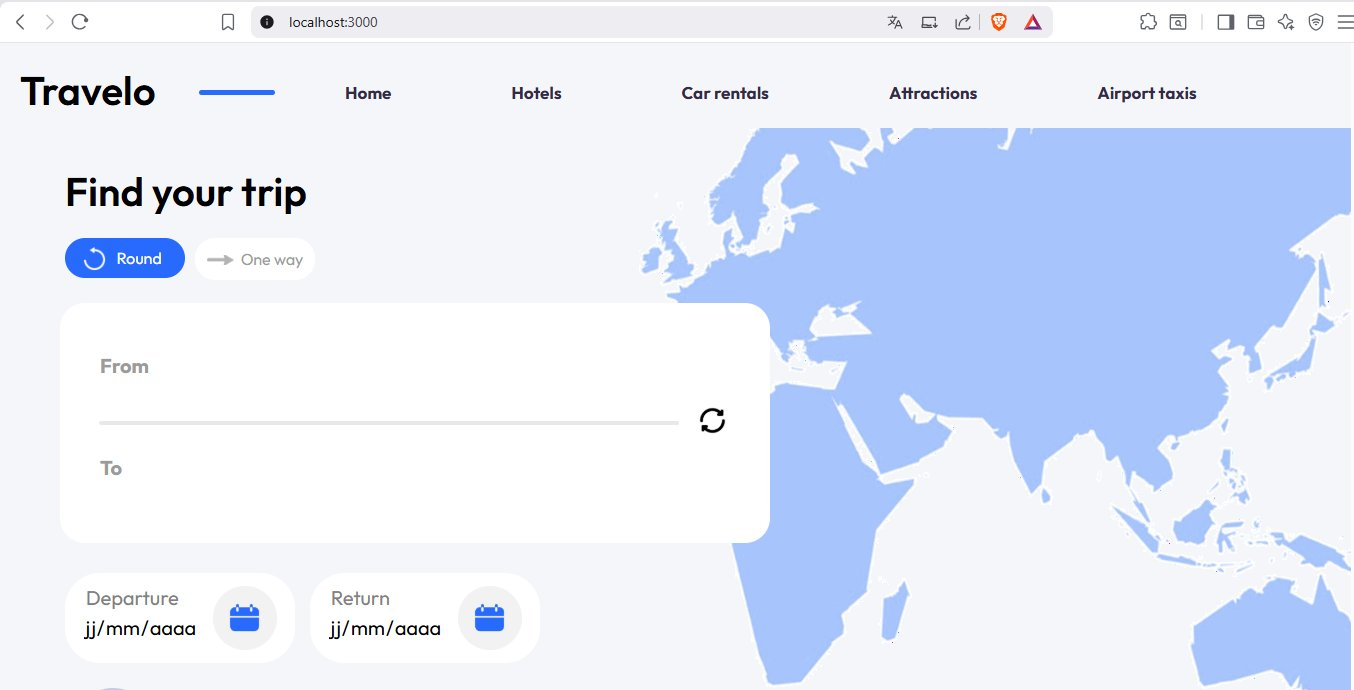
\includegraphics[width=0.95\textwidth]{./screenshots/volet1/55_travelo_accessible_localhost_3000_docker_swarm.png}
    \caption{Application Travelo accessible sur localhost:3000 via Docker Swarm}
\end{figure}

\subsubsection{État détaillé des tâches par service}

\begin{lstlisting}[language=bash]
docker service ps travelo_swarm_backend
docker service ps travelo_swarm_frontend
docker service ps travelo_swarm_mysql
\end{lstlisting}

\begin{figure}[H]
    \centering
    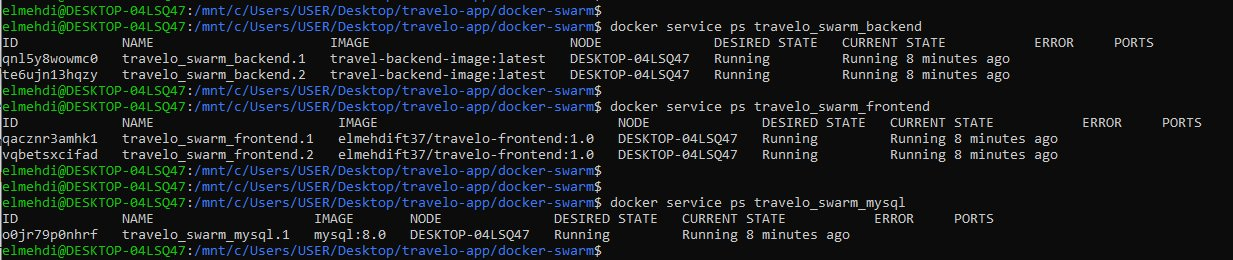
\includegraphics[width=0.95\textwidth]{./screenshots/volet1/56_docker_service_ps_backend_frontend_mysql_running.png}
    \caption{\texttt{docker service ps} : backend (2 tâches Running), frontend (2 tâches Running), mysql (1 tâche Running)}
\end{figure}



\subsection{Conclusion}

Le Volet 1 du projet a permis de conteneuriser et déployer avec succès l'application Travelo selon plusieurs modalités :

\begin{itemize}
    \item \textbf{Conteneurisation individuelle avec Docker} (réseau bridge, volumes, multi-stage builds, scan Trivy)
    \item \textbf{Déploiement orchestré via Docker Compose} (gestion des dépendances, restart policy)
    \item \textbf{Publication sur Docker Hub} (registre public) et sur un \textbf{registre privé local} (registry:2 + UI)
    \item \textbf{Redéploiement depuis le registre privé} avec Docker Compose
    \item \textbf{Bonus : Déploiement en cluster Docker Swarm} avec réplicas (haute disponibilité), limites de ressources, restart policy et reverse proxy Traefik
\end{itemize}

L'application est pleinement opérationnelle dans toutes ces configurations, comme attesté par les captures d'écran du navigateur (localhost:3000).



*Page 21 / 21*
\FloatBarrier
